\documentclass[9pt,twoside,lineno]{pnas-new_SI}
% Use the lineno option to display guide line numbers if required.

\templatetype{pnassupportinginfo}

\usepackage{amsmath}
\usepackage{array} % Required for m{} column
% \usepackage{amssymb}

\newcommand{\CS}{\mathrm{CS}}
\newcommand{\INCB}{\mathrm{INCB}}
\newcommand{\IITT}{\operatorname{IITT}}
\newcommand{\ICS}{\operatorname{ICS}}

\newcommand{\intl}{\int\limits}
\newcommand{\suml}{\sum\limits}
\newcommand{\dd}[1]{\,\mathrm{d}#1}

\renewcommand{\vec}[1]{\mathbf{#1}}
\newcommand{\tens}[1]{\mathrm{#1}}
\newcommand{\itPhi}{\mathit{\Phi}}

% SI units
\usepackage{siunitx}
\DeclareSIUnit\year{yr}
\DeclareSIUnit\carbon{C}

% unit commands
\newcommand{\PgC}{\,\si{\peta\gram\carbon}}
\newcommand{\PgCyr}{\si{\peta\gram\carbon}\,\si{\year}}
\newcommand{\PgCperyr}{\si{\peta\gram\carbon}\,\si{\year}^{-1}}

% eqref with square brackets - shouldn't this work automatically by the chosen style?
\renewcommand{\eqref}[1]{Eq.~[\ref{#1}]}

% eqref without "Eq."
\newcommand{\noEqref}[1]{[\ref{#1}]}

% vector norm
\newcommand{\vnorm}[1]{\left\|#1\right\|}


\title{Tradeoffs between carbon assimilation and release reveal a key role of the tropics in long-term global-scale carbon sequestration}
\author{Estefanía Muñoz, Holger Metzler, Marcos Fernández-Martínez, Jacob A. Nelson, Michael O'Sullivan, Stephen Sitch, Tobias Nützel, George Hurtt, Lei Ma, Qing Sun, Patrick C. McGuire, Etsushi Kato, Xiaojuan Yang and Carlos A. Sierra}

%\author{Muñoz et al. }

\correspondingauthor{E. Muñoz \\E-mail: ehoyos@bgc-jena.mpg.de}


\begin{document}

\renewcommand{\thesection}{S\arabic{section}}
% \renewcommand{\thesubsection}{\thesection.\arabic{section}}
%\numberwithin{equation}{section}

%% Comment out or remove this line before generating final copy for submission; this will also remove the warning re: "Consecutive odd pages found".
%\instructionspage  

\maketitle

%% Adds the main heading for the SI text. Comment out this line if you do not have any supporting information text.

%\setcounter{figure}{0}

%\renewcommand{\tablename}{Supplementary Table}
%\setcounter{table}{0}

%\numberwithin{equation}{section}
%\numberwithin{figure}{section}
%\numberwithin{table}{section}
\SItext


% \subsection*{Subhead}
% Type or paste text here. This should be additional explanatory text such as an extended technical description of results, full details of mathematical models, etc.  

\section{Carbon Sequestration CS and transit times}
The concept of carbon sequestration in ecosystems is closely linked to the concept of the transit time of carbon. In terrestrial ecosystems, we define the transit time of carbon as the amount of time that it takes for carbon atoms to pass through an entire ecosystem, from photosynthesis until respiration by autotrophs and heterotrophs. 
%At a particular time $t$, the time a certain amount of carbon has remained in the system since its arrival at time $t'$ is its age $a=t-t'$.
Because carbon sequestration is not only about the amount of carbon that enters an ecosystem but also about how long it remains stored there, we need an approach that quantifies and combines transit times with the amount of carbon entering ecosystems. Previous works by Sierra et al. \cite{Sierra2021} and Metzler et al. \cite{Metzler2024} introduced a set of definitions integrating transit times with carbon mass. 
Here, we present the connections between transit time and carbon mass, with $\CS$ as used here, and their underlying theory in carbon transit times.


\subsection*{The terrestrial biosphere as a non-autonomous compartmental system}
We can model the carbon stocks and fluxes within, into, and from the terrestrial biosphere as a $d$-dimensional non-autonomous compartmental system that can be described by the vector-valued ordinary differential equation (ODE) 
\begin{equation}
    \label{eqn:comp_sys}
    \begin{aligned}
        \frac{\mathrm{d}}{\dd{t}}\,\vec{C}(t) &= \tens{B}(t)\,\vec{C}(t) + \vec{s}(t),\quad t>t_0,\\
        \vec{C}(t_0) &= \vec{C}_0,
    \end{aligned}
\end{equation}
where $\vec{C}(t)$ is the vector of carbon stocks at time $t$ in $\PgC$ with initial value $\vec{C}_0$ at initial time $t_0$, and $\vec{s}(t)$ is the vector of carbon input fluxes to the terrestrial biosphere coming from the atmosphere at time $t$ in $\PgCperyr$.
The compartmental-matrix-valued function $\tens{B}$ governs the carbon dynamics among the different compartments and carbon leaving the system.
Writing $\vec{1}^T$ for the row vector comprising only ones,
\begin{equation}
    \vec{r}(t) = -\vec{1}^T\,\tens{B}(t)\,\vec{C}(t)
\end{equation}
is the vector of carbon output fluxes from the terrestrial biosphere to the atmosphere at time $t$ in $\PgCperyr$.
The solution to \eqref{eqn:comp_sys} is given by
\begin{equation}
    \vec{C}(t) = \tens{\Phi}(t,t_0)\,\vec{C}_0 + \intl_{t_0}^t \tens{\Phi}(t,t')\,\vec{s}(t')\dd{t'},\quad t\geq t_0,
\end{equation}
with $\tens{\Phi}$ being the state transition operator of the compartmental system.
It is given as the solution to the matrix-valued ODE
\begin{equation}
    \begin{aligned}
        \frac{\mathrm{d}}{\dd{t}}\,\tens{\Phi}(t, t') &= \tens{B}(t)\,\tens{\Phi}(t, t'),\quad t>t',\\
        \tens{\Phi}(t',t') &= \tens{I}_d,
    \end{aligned}
\end{equation}
where $\tens{I}_d$ is the $d$-dimensional identity matrix.
The vector $\tens{\Phi}(t,t')\,\vec{s}(t')$ is the carbon vector of the system input $\vec{s}(t')$ at time $t'$ that is still in the system at time $t$.
Using the $l_1$-norm $\vnorm{\vec{v}} = \sum_{i=d}^d |v_i|$, the scalar functions $C(t):=\vnorm{\vec{C}(t)}$, $s(t):=\vnorm{\vec{s}(t)}$, $r(t):=\vnorm{\vec{r}(t)}$, and the nonnegative value $C_0=\vnorm{\vec{C}_0 }$ describe the total amounts of carbon stocks in the system, the total carbon influx to the system, the total carbon outflux from the system at time $t$, and the total initial carbon stock, respectively.

\subsection*{System sojourn time}
If we define
\begin{equation}
    \itPhi(t,t', \vec{s}) := \tens{\Phi}(t, t')\,\vec{s}
\end{equation}
with $\tens{\Phi}$ being the state transition operator of system in Eq.~\noEqref{eqn:comp_sys}, then $\itPhi(t, t', \vec{s})$ is the amount of the system input $s:=s(t')=\vnorm{\vec{s}(t')}$ at time $t'\leq t$ that is still in the system at time $t$.
Furthermore, $\itPhi$ is linear in $\vec{s}$ such that
\begin{equation}
    \itPhi(t,t,',\vec{s_1}+\vec{s_2}) = \itPhi(t,t',\vec{s_1}) + \itPhi(t,t',\vec{s_2}).
\end{equation}
Now, divide $\vec{s}$ into $N$ equally small packages $\vec{s}_i=\vec{s}/N$ such that $\vec{s}=\sum_{i=1}^N \vec{s}_i$.
We make the packages $\vec{s}_i$ so small by choosing $N$ so large such that, for all $i\leq N$ and all $t\geq t'$, we have
\begin{equation}
    \itPhi(t, t', \vec{s}_i) = \Psi_i(t, t') \, s_i
\end{equation}
with $s_i=\vnorm{\vec{s}_i}$ and $\Psi_i(t, t') \in \{0, 1\}$.
This means that all particles of $s_i$ show the same future behavior after $t'$ in the sense that
\begin{equation}
    \mathit{\Psi}_i(t, t') = 
    \begin{cases}
        0, & \text{all particles of $s_i$ have left the system before time }t,\\
        1, & \text{all particles of $s_i$ are still in the system at time }t.
    \end{cases}
\end{equation}
By construction,
\begin{equation}
    \intl_{t'}^{t_0+T} \Psi_i(t, t')\dd{t}
\end{equation}
is the time that a single particle of $s_i$ spends in the system during the interval $[t',t_0+T]$ and
\begin{equation}
    s_i\intl_{t'}^{t_0+T} \Psi_i(t, t')\dd{t}
\end{equation}
is the mass-time ($\PgCyr$) that $s_i$ spends in the system.
Consequently,
\begin{equation}
    \begin{aligned}
        \intl_{t'}^{t_0+T} \itPhi(t',t,\vec{s}(t'))\dd{t} &= \intl_{t'}^{t_0+T} \itPhi\left(t,t',\sum_{i=1}^N \vec{s}_i\right)\dd{t}
        &= \intl_{t'}^{t_0+T} \sum_{i=1}^N \itPhi(t,t',\vec{s}_i)\dd{t}
        &= \intl_{t'}^{t_0+T} \sum_{i=1}^N \Psi_i(t,t')\,s_i\dd{t}\\
        &= \sum_{i=1}^N s_i\intl_{t'}^{t_0+T}\Psi_i(t,t')\dd{t}
    \end{aligned}
\end{equation}
describes the mass-time ($\PgCyr$) that all particles of the input $\vec{s}(t')$ spend in the system during the interval $[t',t_0+T]$.
We call this mass-time $\itPhi(t,t',\vec{s}(t'))$ the \emph{system sojourn time} of $s(t')$.

\subsection*{Carbon sequestration, system sojourn times, and transit times of compartmental systems}
In this section, we show how our definition of $\CS$ is related to the concepts 
\emph{Integrated Net Carbon Balance} ($\INCB$), \emph{Integrated Inputs Transit Time} ($\IITT$), and \emph{Integrated Carbon Stocks} ($\ICS$) introduced in Metzler et al. \cite{Metzler2024} and of which $\IITT$ is equivalent to \emph{Carbon Sequestration} ($\CS$) as defined (differently from here) in Sierra et al. \cite{Sierra2021}.
Except for $\INCB$, all of these concepts are connected to each other through the underlying concepts of system sojourn times or transit times.
Unfortunately, despite its lack of support by transit times, $\INCB$ is very often used as a metric for carbon sequestration.

More generally, we want to demonstrate that a family of metrics can effectively integrate the concepts of carbon inputs and transit times, allowing us to quantify the more general concept of carbon sequestration (Table~\ref{Table:family_of_measures}).
The aspects of the general theory of forward transit times of non-autonomous compartmental systems that we present here originate from Metzler et al. \cite{Metzler2018PNAS}.

The forward transit time $\tau(t')$ of a non-autonomous compartmental system is the time span that input entering the system at time $t'$ will spend in it before exiting.
The exit occurs at time $t$, with the particle's age at exit given by $a=t-t'$, where age measures the time since the particle's entry into the system.
This forward transit time has a density function $p_\tau(\cdot,t')$ such that $p_\tau(t-t',t')$ is the mass that enters the system at time $t'$ and leaves the system at time $t$, having spent the period $a=t-t'$ in the system.

For the compartmental system in Eq.~\noEqref{eqn:comp_sys}, the density is given by
\begin{equation}
    p_\tau(t-t', t') = -\vec{1}^T\,\tens{B}(t)\,\tens{\Phi}(t, t')\,\vec{s}(t')
\end{equation}
and its cumulative distribution by
\begin{equation}
    \begin{aligned}
        P_\tau(t-t',t') &= \intl_0^{t-t'} p_\tau(a, t')\dd{a} = \vnorm{\vec{s}(t')} - \vnorm{\tens{\Phi}(t,t')\,\vec{s}(t')} \\
        &= s(t') - \itPhi(t,t',\vec{s}(t')).
    \end{aligned}
\end{equation}
The cumulative distribution $P_\tau(t-t',t')$ describes the mass that enters the system at time $t'$ and leaves the system before an age smaller than $t-t'$, hence before $t'$.
The survival function
\begin{equation}
    S_\tau(t-t',t'):=\vnorm{\vec{s}(\tau)} - P_\tau(t-t',t') = \vnorm{\tens{\Phi}(t,t')\,\vec{s}(t')} = \itPhi(t,t',\vec{s}(t'))
\end{equation}
describes the remaining amount at time $t$ from the input at time $t'$.
To make $p_\tau(\cdot,t')$, $P_\tau(\cdot,t')$, and $S_\tau(\cdot,t')$ probability density functions, cumulative distribution functions, and probabilistic survival functions, we need to normalize them by the total input amount $s(t')$ at time $t'$.
Defining $\vec{\beta}(t'):=\vec{s}(t')/s(t')$ to be the unit vector (in $l_1$-norm) that distributes the incoming carbon $s(t')$ at time $t$ to the different compartments, we obtain the normalized cumulative distribution function of $\tau(t')$ as
\begin{equation}
    F_\tau(t-t',t') = 1 - \vnorm{\tens{\Phi}(t,t')\,\vec{\beta}(t')}
\end{equation}
and its mean or expected value as
\begin{equation}
    \mathbb{E}\left[\tau(t')\right] = \intl_{t'}^\infty \left[1-F_\tau(t-t',t')\right]\dd{t} = \intl_{t'}^\infty \vnorm{\tens{\Phi}(t,t')\,\vec{\beta}(t')}\dd{t},
\end{equation}
and hence
\begin{equation}
    \intl_{t'}^\infty \vnorm{\tens{\Phi}(t,t')\,\vec{s}(t')}\dd{t} = s(t')\,\mathbb{E}\left[\tau(t')\right]
\end{equation}
as a weighted mean transit time.
Recalling $\itPhi(t,t',\vec{s}(t'))=\vnorm{\tens{\Phi}(t,t')\,\vec{s}(t')}$, we can interpret the system sojourn time of
$s(t')$, given by
\begin{equation}
    \intl_{t'}^{t_0+T} \itPhi(t,t',\vec{s}(t'))\dd{t} = \int_{t'}^{t_0+T} \vnorm{\tens{\Phi}(t,t')\,\vec{s}(t')}\dd{t},
\end{equation}
as a weighted \emph{truncated mean forward transit time}.

Consequently, the \emph{Integrated Inputs Transit Time} on the interval $[t_0, t_0+T]$, defined as
\begin{equation}
    \label{eqn:IITT}
    \IITT(t_0, T) := \intl_{t_0}^{t_0+T} \intl_{t'}^{t_0+T} \vnorm{\tens{\Phi}(t,t')\,\vec{s}(t')}\dd{t}\dd{t'} = \intl_{t_0}^{t_0+T} \intl_{t'}^{t_0+T} \itPhi(t,t',\vec{s}(t'))\dd{t}\dd{t'},
\end{equation}
represents the integrated weighted truncated mean forward transit times or the integrated system sojourn times of inputs to the system on the interval $[t_0, t_0+T]$.

$\IITT$ considers only the fate of carbon input to the system during the interval $[t_0,t_0+T]$ and ignores the fate of the initial carbon vector $\vec{C}_0$.
If we interpret $\vec{C}_0$ as a pulse input $\delta(t'-t_0)\,\vec{C}_0$ at time $t_0$, then we can extend $\IITT$ to
\begin{equation}
    \label{eqn:ICS}
    \begin{aligned}
        \intl_{t_0}^{t_0+t} \intl_{t'}^{t_0+T} &\vnorm{\tens{\Phi}(t,t')\,\left[s(t') + \delta(t'-t_0)\,\vec{C}_0\right]}\dd{t}\dd{t'} \\
        &=\intl_{t_0}^{t_0+T} \delta(t'-t_0) \intl_{t'}^{t_0+T}\vnorm{\tens{\Phi}(t,t')\,\vec{C}_0}\dd{t}\dd{t'} + \intl_{t_0}^{t_0+T}\intl_{t'}^{t_0+T}\vnorm{\tens{\Phi}(t,t')\,\vec{s}(t')}\dd{t}\dd{t'}\\
        &= \intl_{t_0}^{t_0+T}\vnorm{\tens{\Phi}(t,t_0)\,\vec{C}_0}\dd{t} +\intl_{t_0}^{t_0+T}\intl_{t'}^{t_0+T}\vnorm{\tens{\Phi}(t,t')\,\vec{s}(t')}\dd{t}\dd{t'}\\
        & = \intl_{t_0}^{t_0+T}\vnorm{\tens{\Phi}(t,t_0)\,\vec{C}_0}\dd{t} + \intl_{t_0}^{t_0+T} \intl_{t_0}^t \vnorm{\tens{\Phi}(t,t')\,\vec{s}(t')}\dd{t'}\dd{t}\\
        &= \int_{t_0}^{t_0+T} \vnorm{\vec{C}(t)}\dd{t},
    \end{aligned}
\end{equation}
which equals the \emph{Integrated Carbon Stocks} $\ICS(t_0,T)$, meaning, we can interpret $\ICS(t_0, T)$ as a weighted system sojourn time of all particles that at some time belong to the system during the interval $[t_0,t_0+T]$ or as weighted truncated mean forward transit time of all particles entering the system with the initial carbon stocks interpreted as a pulse input.

Considering the \emph{Integrated Net Carbon Balance}
\begin{equation}
    \INCB(t_0,t) = \intl_{t_0}^{t}\left[\vnorm{\vec{s}(t')}-\vnorm{\vec{r}(t')}\right]\dd{t'} = \intl_{t_0}^t \left[s(t')-r(t')\right]\dd{t'} = C(t)-C_0,
\end{equation}
we notice that the \emph{Carbon Sequestration}
\begin{equation}
    \CS(t_0,T) = \intl_{t_0}^{t_0+T} \intl_{t_0}^t \left[s(t')-r(t')\right]\dd{t'}\dd{t}
\end{equation}
can be written as
\begin{equation}
    \CS(t_0,T) = \intl_{t_0}^{t_0+T} \INCB(t_0,t)\dd{t} = \intl_{t_0}^{t_0+T} \left[C(t) - C_0\right]\dd{t} = \ICS(t_0,T) - T\,C_0.
\end{equation}
Notice that if we start with an empty system, i.e., $\vec{C}(t_0) = \vec{0}$, all metrics coincide, i.e.,  $\CS = \ICS = \IITT$. 
Similarly, if we compare $\CS$ for two different scenarios $A$ and $B$, both with the same initial condition $\vec{C}(t_0)=\vec{C}_0$, then
\begin{equation}
    \label{eqn:Delta_CS}
    \Delta\CS(A,B) := \CS_A(t_0,T) - \CS_B(t_0,T) = \ICS_A(t_0,T) - \ICS_B(t_0,T)
\end{equation}
and hence $\Delta\CS(A,B)$ is a comparison measure of two scenarios $A$ and $B$ based on weighted system sojourn times or weighted truncated mean forward transit times.

In summary, the family of metrics IITT, ICS, and CS are different forms of mean forward transit times integrated over time and truncated until the time of observation. Their main difference is the way they treat the legacy carbon from the initial conditions. One of the main advantages of using these metrics is that they combine both the amount of carbon and the time it remains stored in a compartmental system without the need to explicitly calculate transit times. We believe these metrics are essential to quantify the more general concept of Carbon Sequestration because they account for how much of the total carbon that enters a system will be retained for a period of time, potentially including legacy effects from previously stored carbon. 


\begin{table}[t]
    \caption{A family of carbon sequestration metrics. $\IITT$ is constructed directly on transit times, $\ICS$ extends $\IITT$ by interpreting the initial stocks as a pulse input, and $\CS$ allows comparison of different scenarios with equal initial total carbon stocks by having only fluxes available. In the case of an empty initial system, $C_0=0$, the three metrics coincide.}
    \begin{center}
        \begin{tabular}{m{3cm} m{4cm} m{4cm} m{4cm}}
            \toprule
            \multicolumn{1}{c}{} & 
            \multicolumn{1}{c}{\textbf{Integrated Inputs Transit Time}} & 
            \multicolumn{1}{c}{\textbf{Integrated Carbon Stocks}} & 
            \multicolumn{1}{c}{\textbf{Carbon Sequestration}} \\
            \midrule
            \vspace{50pt}
            \textbf{Computation} &
                $\begin{array}{c}
                    \displaystyle \IITT(t_0,T) \\
                    \displaystyle =\intl_{t_0}^{t_0+T} \intl_{t'}^{t_0+T} \vnorm{\tens{\Phi}(t,t')\,\vec{s}(t')}\dd{t}\dd{t'} \\
                    \displaystyle = \intl_{t_0}^{t_0+T} \intl_{t'}^{t_0+T} \itPhi(t,t',s(t'))\dd{t}\dd{t'}\\
                    \displaystyle = \ICS - \intl_{t_0}^{t_0+T} \vnorm{\tens{\Phi}(t,t_0)\,\vec{C}_0}\dd{t}
                \end{array}$
             &
                $\begin{array}{c}
                    \displaystyle \ICS(t_0,T) \\
                    \displaystyle =\intl_{t_0}^{t_0+T} \vnorm{\vec{C}(t)}\dd{t} \\
                    \displaystyle  =\intl_{t_0}^{t_0+T} C(t)\dd{t} \\
                    \displaystyle = \IITT + \intl_{t_0}^{t_0+T} \vnorm{\tens{\Phi}(t,t_0)\,\vec{C}_0}\dd{t}
                \end{array}$
                &
                $\begin{array}{c}
                    \displaystyle \CS(t_0,T) \\
                    \displaystyle =\intl_{t_0}^{t_0+T} \intl_{t_0}^t \left[s(t')-r(t')\right]\dd{t'} \dd{t} \\
                    \displaystyle =\intl_{t_0}^{t_0+T} \left[C(t) - C_0\right]\dd{t} \\
                    \displaystyle =\ICS - T\,C_0 \vphantom{\intl_{t_0}^{t_0+T}}
                \end{array}$ \\
            \hline
            \textbf{Computational requirements} & 
            \begin{itemize}
                \item State transition operator $\tens{\Phi}$ and influx vector $\vec{s}(t)$ through time. 
                \item Or $\ICS$ requirements and state transition operator $\tens{\Phi}$ through time.
            \end{itemize} &
            \begin{itemize}
                \item Total carbon stocks $C(t)$ through time. 
                \item Or $\IITT$ requirements and total initial carbon stocks $C(t_0)$.
            \end{itemize} &
            \begin{itemize}
                \item Total influx amounts $s(t)$ and total outflux amounts $r(t)$ through time. 
                \item Or total net influx through time.
                \item Or total carbon stocks $C(t)$ through time.
            \end{itemize} \\
            \hline
            \textbf{Connection to transit times} & 
            Directly by construction as shown in~\eqref{eqn:IITT}. & 
            By interpretation as $\IITT$ extended to the initial stock vector $\vec{C_0}$ as a pulse input. & 
            By relative comparison in a scenario setup as shown in~\eqref{eqn:Delta_CS}. \\
            \bottomrule
        \end{tabular}
    \end{center}
    \label{Table:family_of_measures}
\end{table}

\section{Product information and data}

\begin{table}[ht]
\centering
\label{Tab:CMIP6models}
\caption{CMIP6 Earth system models included in this study and relevant features.}
\begin{tabular}{llccccccl}
\textbf{\begin{tabular}[c]{@{}l@{}}Earth system\\  model\end{tabular}} & \textbf{\begin{tabular}[c]{@{}l@{}}Modelling \\ centre\end{tabular}} & \multicolumn{1}{l}{\textbf{NEP}} & \multicolumn{1}{l}{\textbf{NBP}} & \multicolumn{1}{l}{\textbf{N cycle}}                     & \multicolumn{1}{l}{\textbf{Fires}}                       & \multicolumn{1}{l}{\textbf{\begin{tabular}[c]{@{}l@{}}Dynamic \\ vegetation\end{tabular}}} & \textbf{\begin{tabular}[c]{@{}l@{}}Land carbon\\ model\end{tabular}}  & \multicolumn{1}{l}{\textbf{Reference}}  \\ \hline
ACCESS-ESM1-5                                                          & CSIRO                                                                & Yes                              & Yes                              & \begin{tabular}[c]{@{}c@{}}Yes \\ (p-cycle)\end{tabular} & No                                                       & No                                                                                         & \begin{tabular}[c]{@{}l@{}}CABLE2.4 with\\ CASA-CNP\end{tabular}   &  Ziehn et al. \cite{ACCESS}  \\
BCC-CSM2-MR                                                            & BCC                                                                  & Yes                              & No                               & No                                                       & No                                                       & No                                                                                         & BCC-AVIM2            & Wu et al. \cite{BCC}                                                \\
CanESM5                                                                & CCCma                                                                & Yes                              & Yes                              & No                                                       & No                                                       & \begin{tabular}[c]{@{}c@{}}Only\\ wetlands\end{tabular}                                    & CLASS-CTEM            & Swart et al. \cite{CanESM5}                                               \\
CESM2                                                                  & CESM                                                                 & No                               & Yes                              & Yes                                                      & Yes                                                      & Yes                                                                                        & CLM5                   & Danabasoglu \cite{CESM2}                                              \\
CNRM-ESM2-1                                                            & CNRM                                                                 & Yes                              & Yes                              & Implicit                                                 & \begin{tabular}[c]{@{}c@{}}Yes \\ (Natural)\end{tabular} & No                                                                                         & ISBA-CTRIP                & Seferian \cite{CNRM}                                           \\
NOAA-GFDL-ESM4                                                         & \begin{tabular}[c]{@{}l@{}}NOAA, \\ GFDL\end{tabular}                & Yes                              & Yes                              & No                                                       & Yes                                                      & Yes                                                                                        & LM4p1              & Krasting et al. \cite{NOAA}                                                 \\
MPI-ESM1-2-LR                                                          & MPI                                                                  & Yes                              & Yes                              & Yes                                                      & Yes                                                      & Yes                                                                                        & JSBACH3.2                & Wieners et al. \cite{MPI}                                            \\
NorESM2-LM                                                             & NCC                                                                  & Yes                              & Yes                              & Yes                                                      & Yes                                                      & No                                                                                         & CLM5              &Seland et al. \cite{NorESM2}\\
UKESM1-0-LL                                                            & UK                                                                   & Yes                              & Yes                              & Yes                                                      & No                                                       & Yes                                                                                        & JULES-ES1.0             & Tang et al. \cite{UKESM}                                             \\ \hline
\end{tabular}
\end{table}



\begin{table}[ht]
\centering
\label{Tab:TRENDYmodels}
\caption{TRENDY models included in this study and relevant features.}
\begin{tabular}{llll}
\textbf{Model} & \textbf{NEP} & \textbf{NBP} & \textbf{Reference}                                                                                                                  \\ \hline
CABLE-POP      & Yes          & Yes          & Haverd et al. (2018)                                                                                                                \\
CLASSIC        & Yes          & Yes          & Melton et al. (2020)                                                                                                                \\
CLM5.0         & Yes          & Yes          & Lawrence et al. (2019)                                                                                                              \\
DLEM           & Yes          & No           & Tian et al. (2015), You et al. (2022)                                                                                               \\
ED             & Yes          & Yes          & Moorcroft et al. (2001), Ma et al. (2022)                                                                                           \\
ELM            & Yes          & Yes          & Yang et al.(2023), Burrows et al. (2020)                                                                                            \\
IBIS           & Yes          & Yes          & Xia et al. (2024)                                                                                                                   \\
iMAPLE         & Yes          & Yes          & Yue et al. (2024)                                                                                                                   \\
ISAM           & Yes          & Yes          & \begin{tabular}[c]{@{}l@{}}Jain et al. (2013), Meiyappan et al. (2015), \\ Shu et al. (2020)\end{tabular}                           \\
ISBA-CTRIP& Yes          & Yes          & Delire et al. (2020)                                                                                                                \\
JSBACH         & Yes          & Yes          & Mauritsen et al. (2019), Reick et al. (2021)                                                                                        \\
JULES          & Yes          & Yes          & \begin{tabular}[c]{@{}l@{}}Wiltshire et al. (2021), Sellar et al. (2019), \\ Burton et al. (2019)\end{tabular}                      \\
LPJml          & Yes          & No           & \begin{tabular}[c]{@{}l@{}}Schaphoff et al. (2018), von Bloh et al. (2018),\\ Lutz et al. (2019), Heinke et al. (2023)\end{tabular} \\
LPJwsl         & Yes          & Yes          & Poulter et al. (2011)                                                                                                               \\
LPX-Bern            & Yes          & Yes          & Lienert and Joos (2018)                                                                                                             \\
OCN            & Yes          & Yes          & Zaehle and Friend (2010), Zaehle et al. (2011)                                                                                      \\
ORCHIDEE       & Yes          & Yes          & \begin{tabular}[c]{@{}l@{}}Krinner et al. (2005), Zaehle and Friend (2010), \\ Vuichard et al. (2019)\end{tabular}                  \\
SDGVM          & Yes          & No           & Woodward and Lomas (2004), Walker et al. (2017)                                                                                     \\
VISIT          & Yes          & Yes          & Ito and Inatomi (2012), Kato et al. (2013)                                                                                          \\
VISIT-UT       & Yes          & Yes          &                                                                                                                                     \\ \hline
\end{tabular}
\end{table}

\clearpage

\begin{figure}[H]
    \centering
    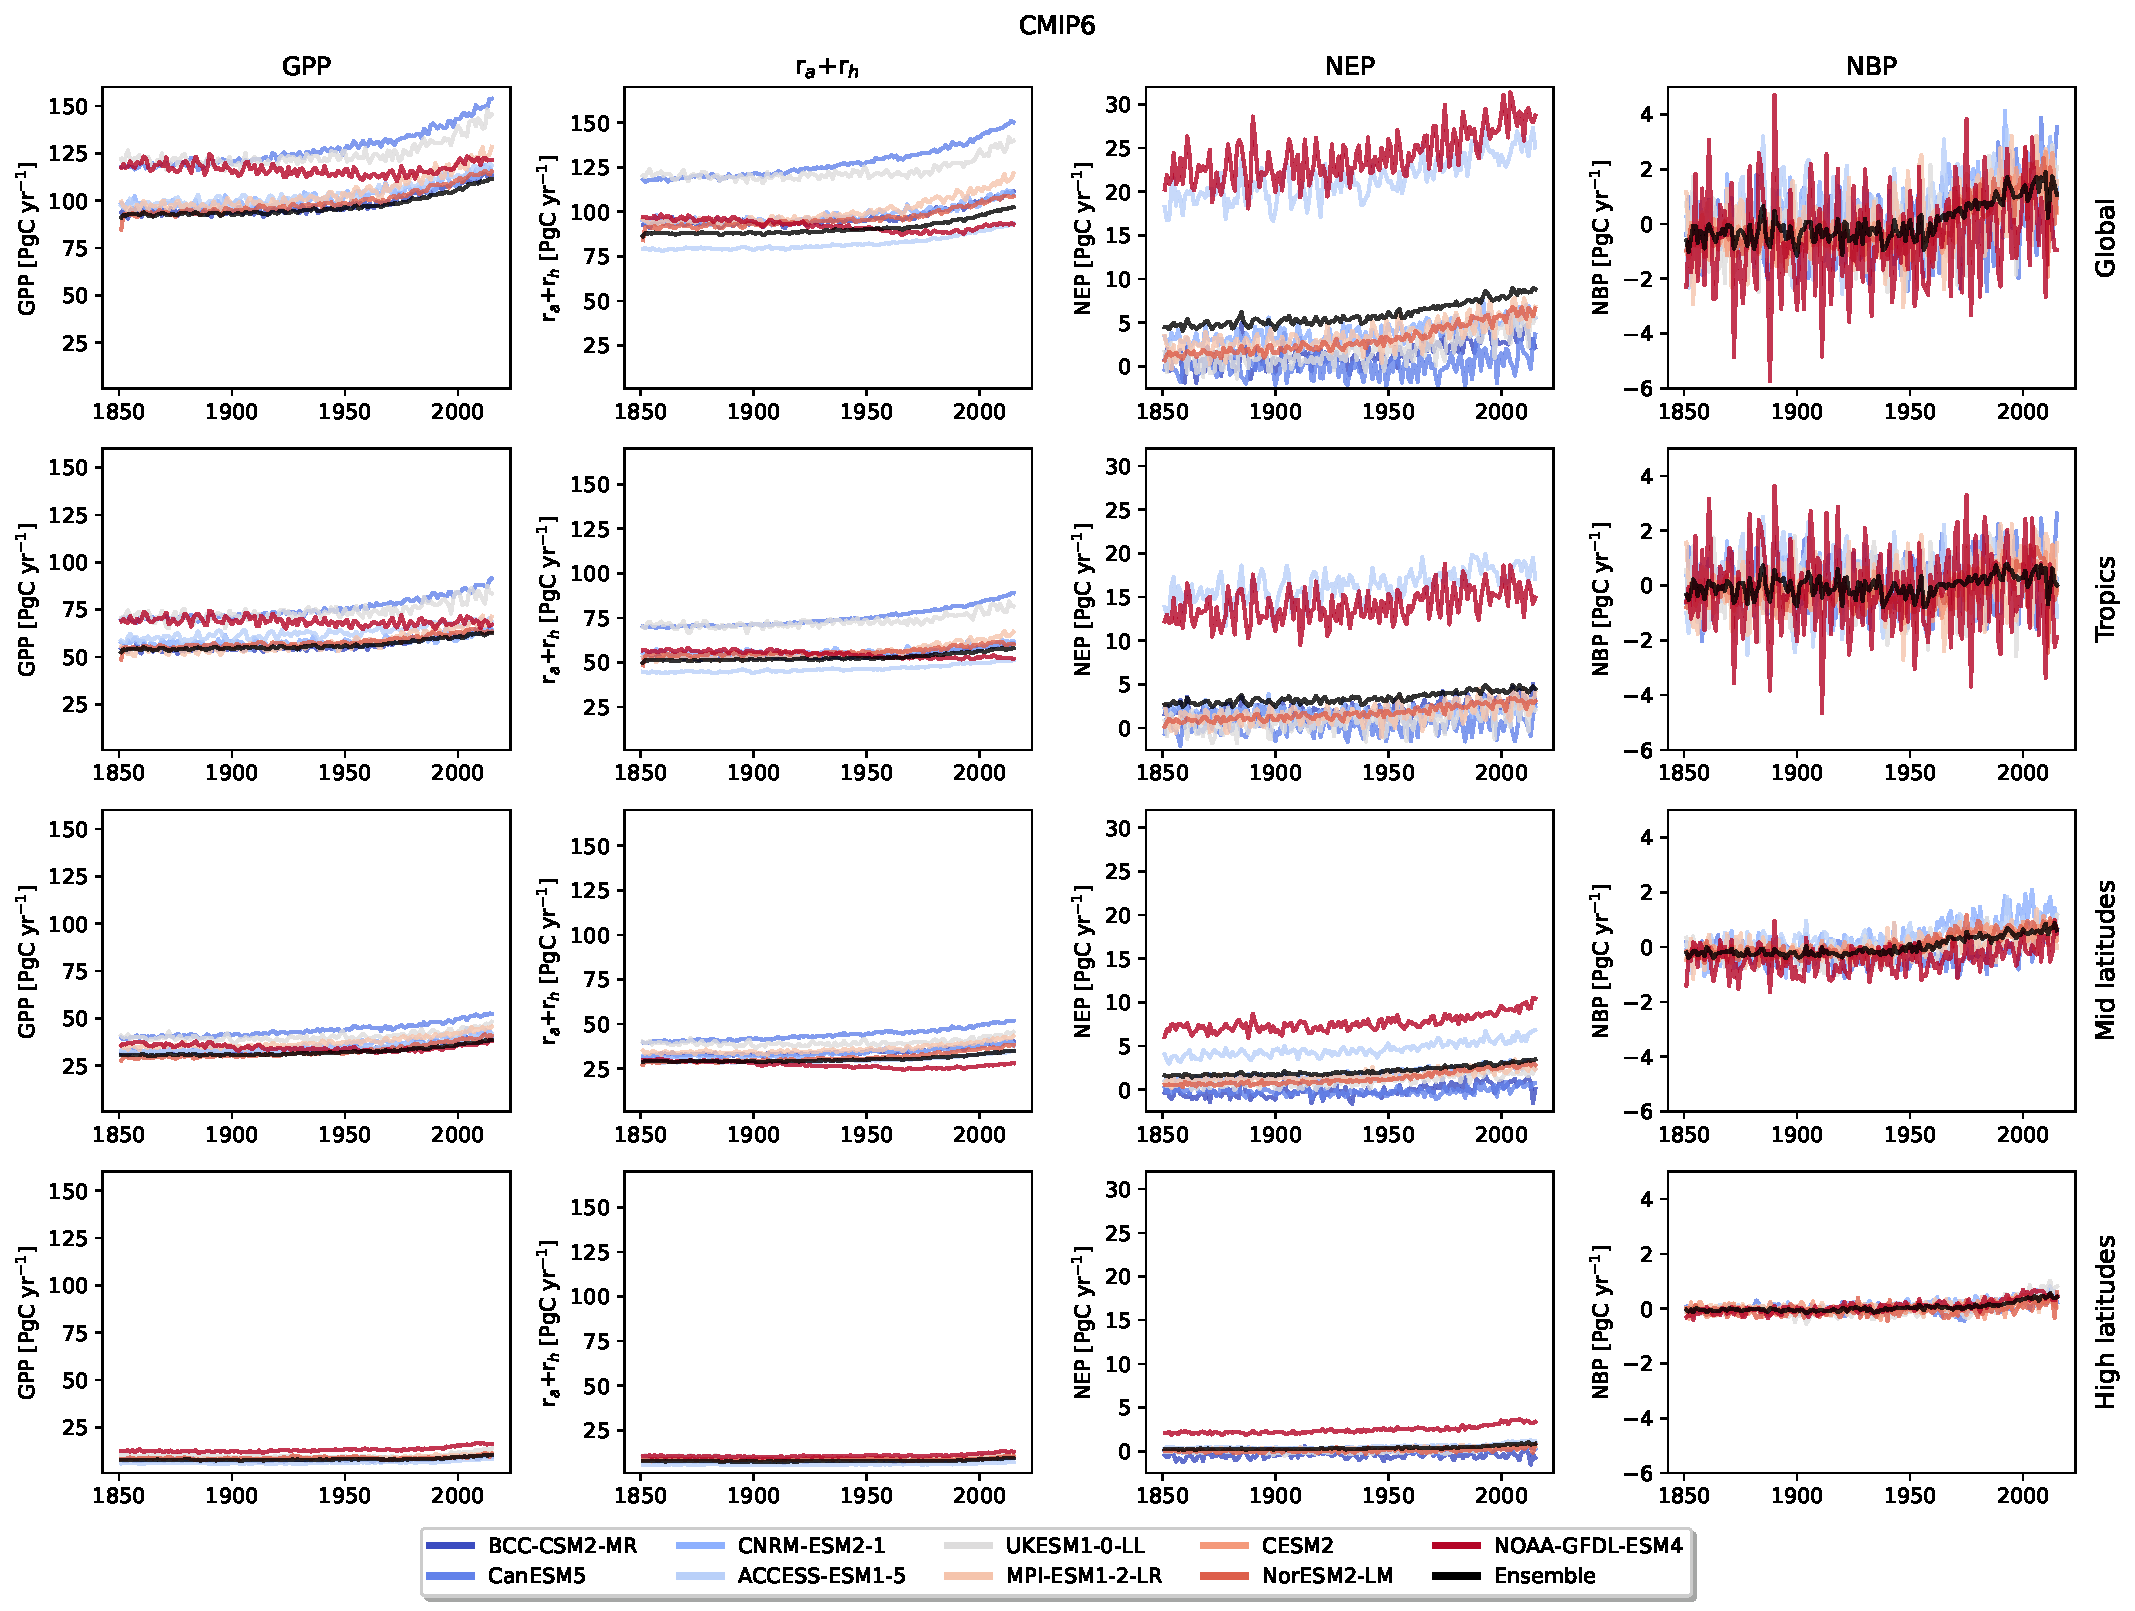
\includegraphics[width=1.0\linewidth]{Figures/CMIP6_variables.pdf}
    \caption{Time series of the annual mean of GPP, total respiration ($r_h+r_a$), NEP and NBP (vertical panels) from CMIP6 models, cumulated globally, in the tropics, mid latitudes, and high latitudes (horizontal panels). Colors indicate the different models and black lines the ensemble.}
    \label{fig:vars_CMIP6}
\end{figure}

\newpage
\begin{figure}[H]
    \centering
    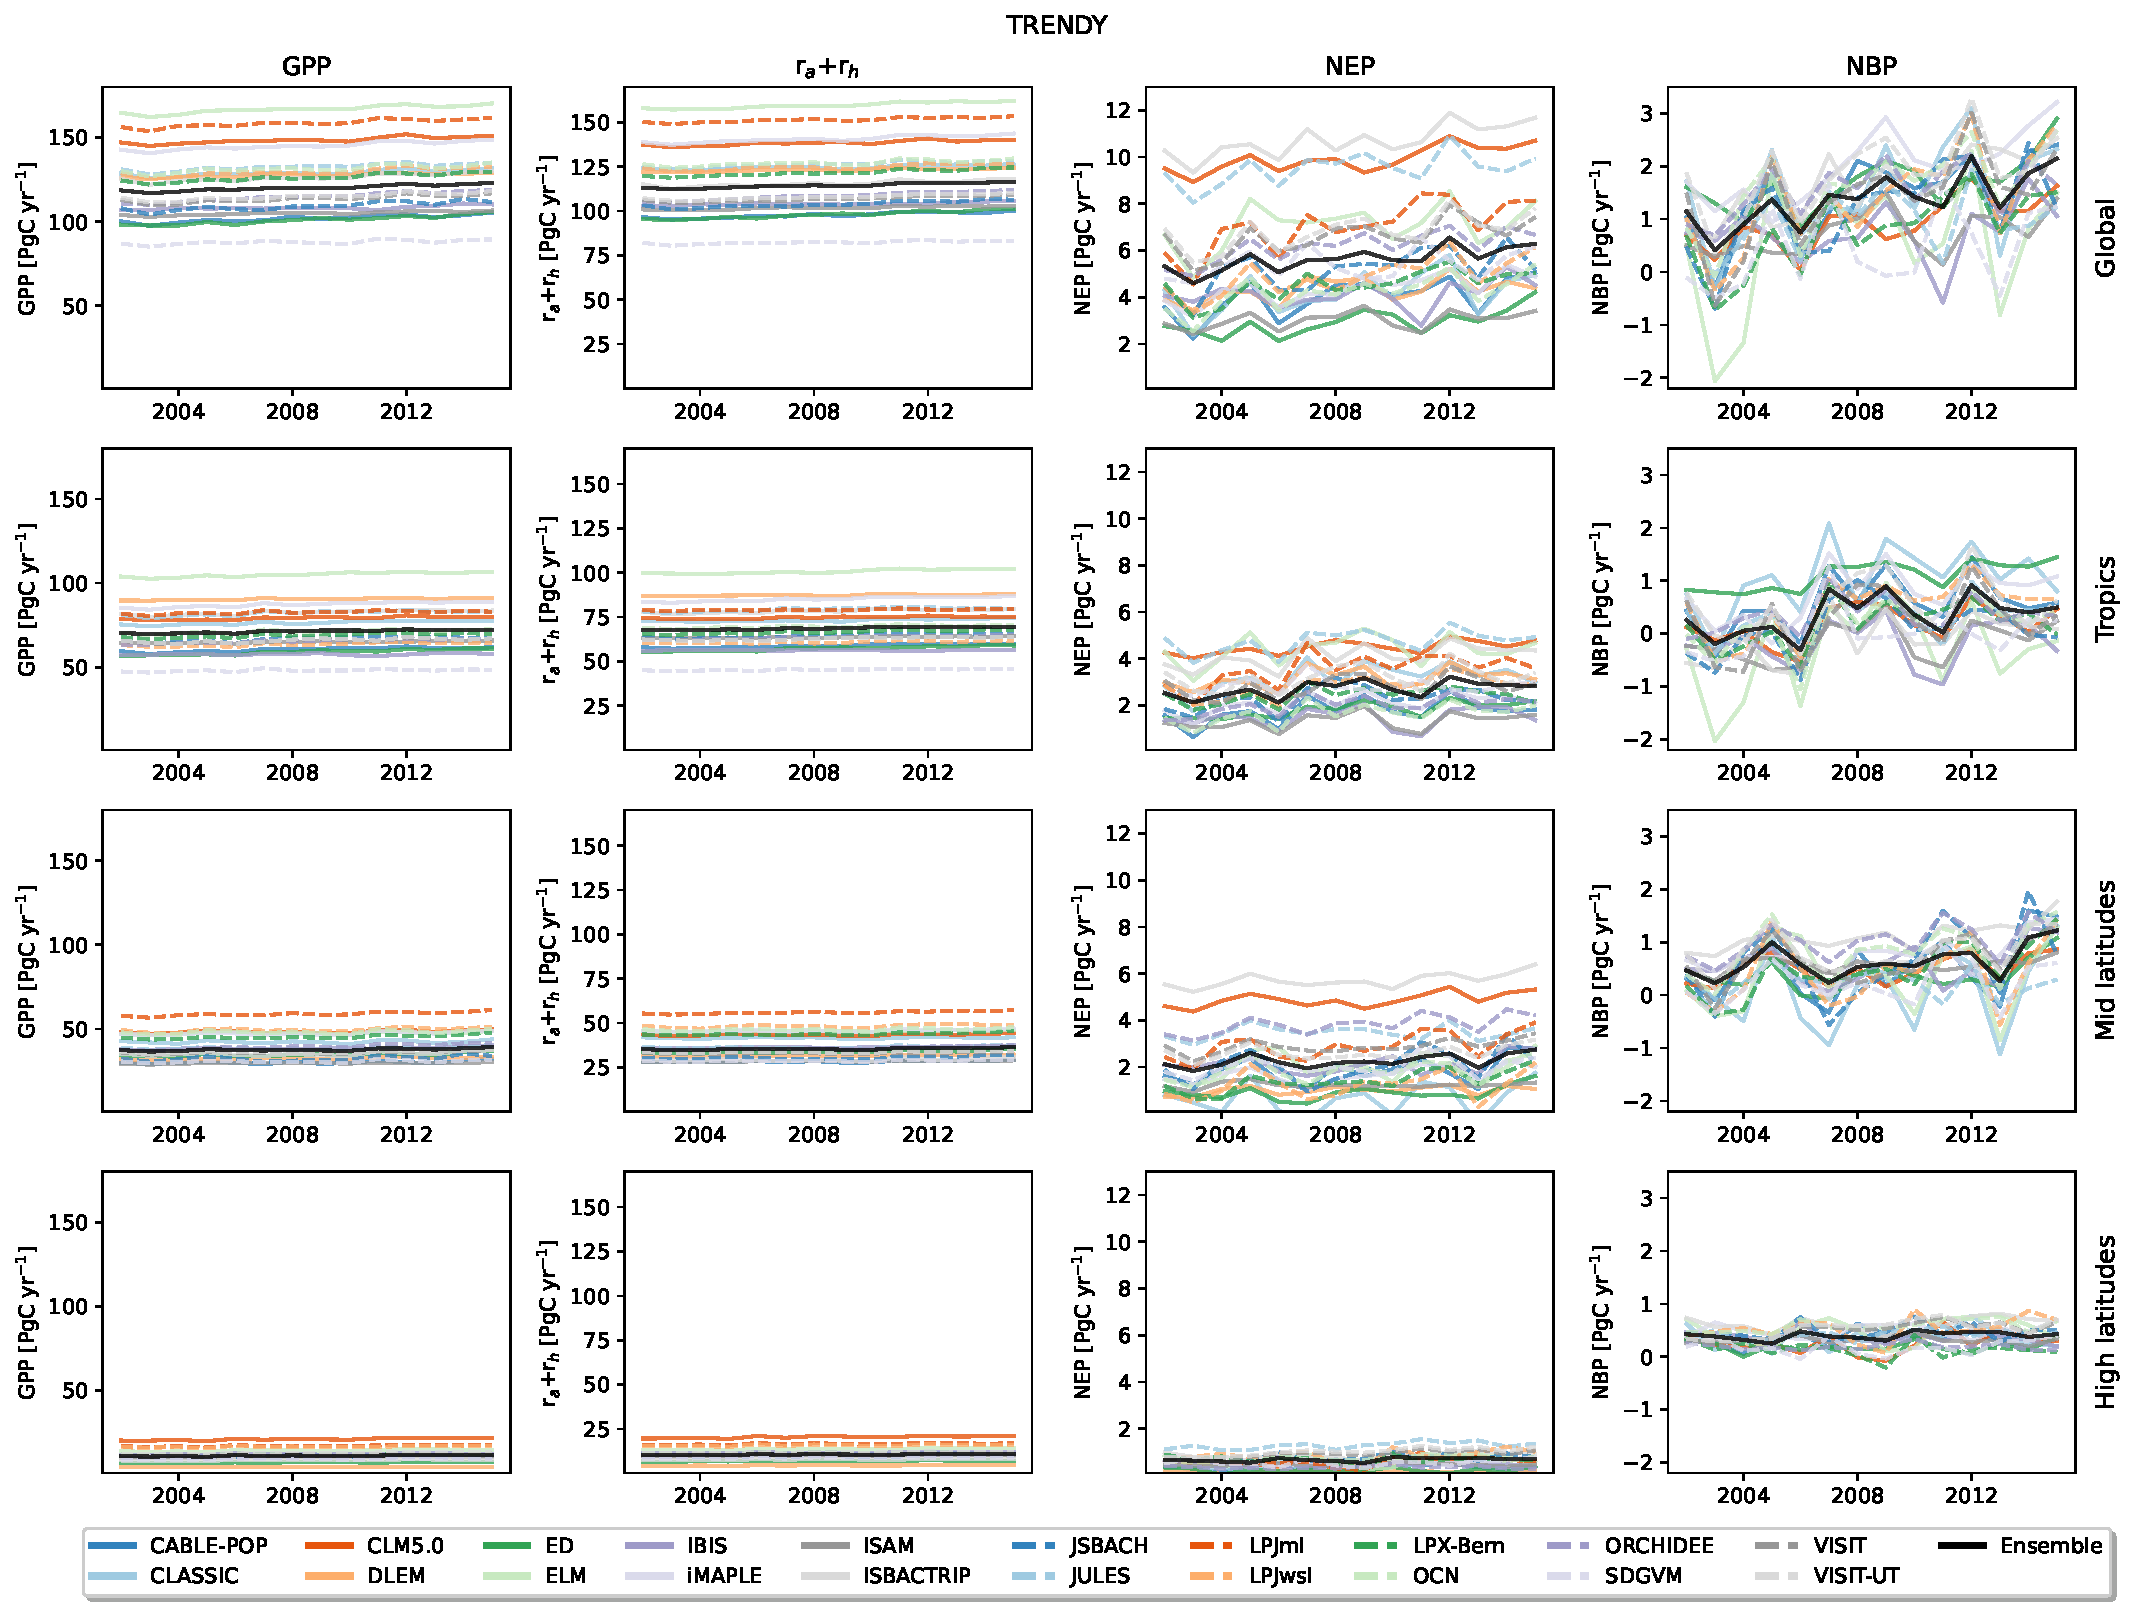
\includegraphics[width=1.0\linewidth]{Figures/TRENDY_variables.pdf}
    \caption{Time series of the annual mean of GPP, total respiration ($r_h+r_a$), NEP and NBP (vertical panels) from TRENDY models, cumulated globally, in the tropics, mid latitudes, and high latitudes (horizontal panels). Colors indicate the different models and black lines the ensemble.}
    \label{fig:vars_TRENDY}
\end{figure}

\newpage
\begin{figure}[H]
    \centering
    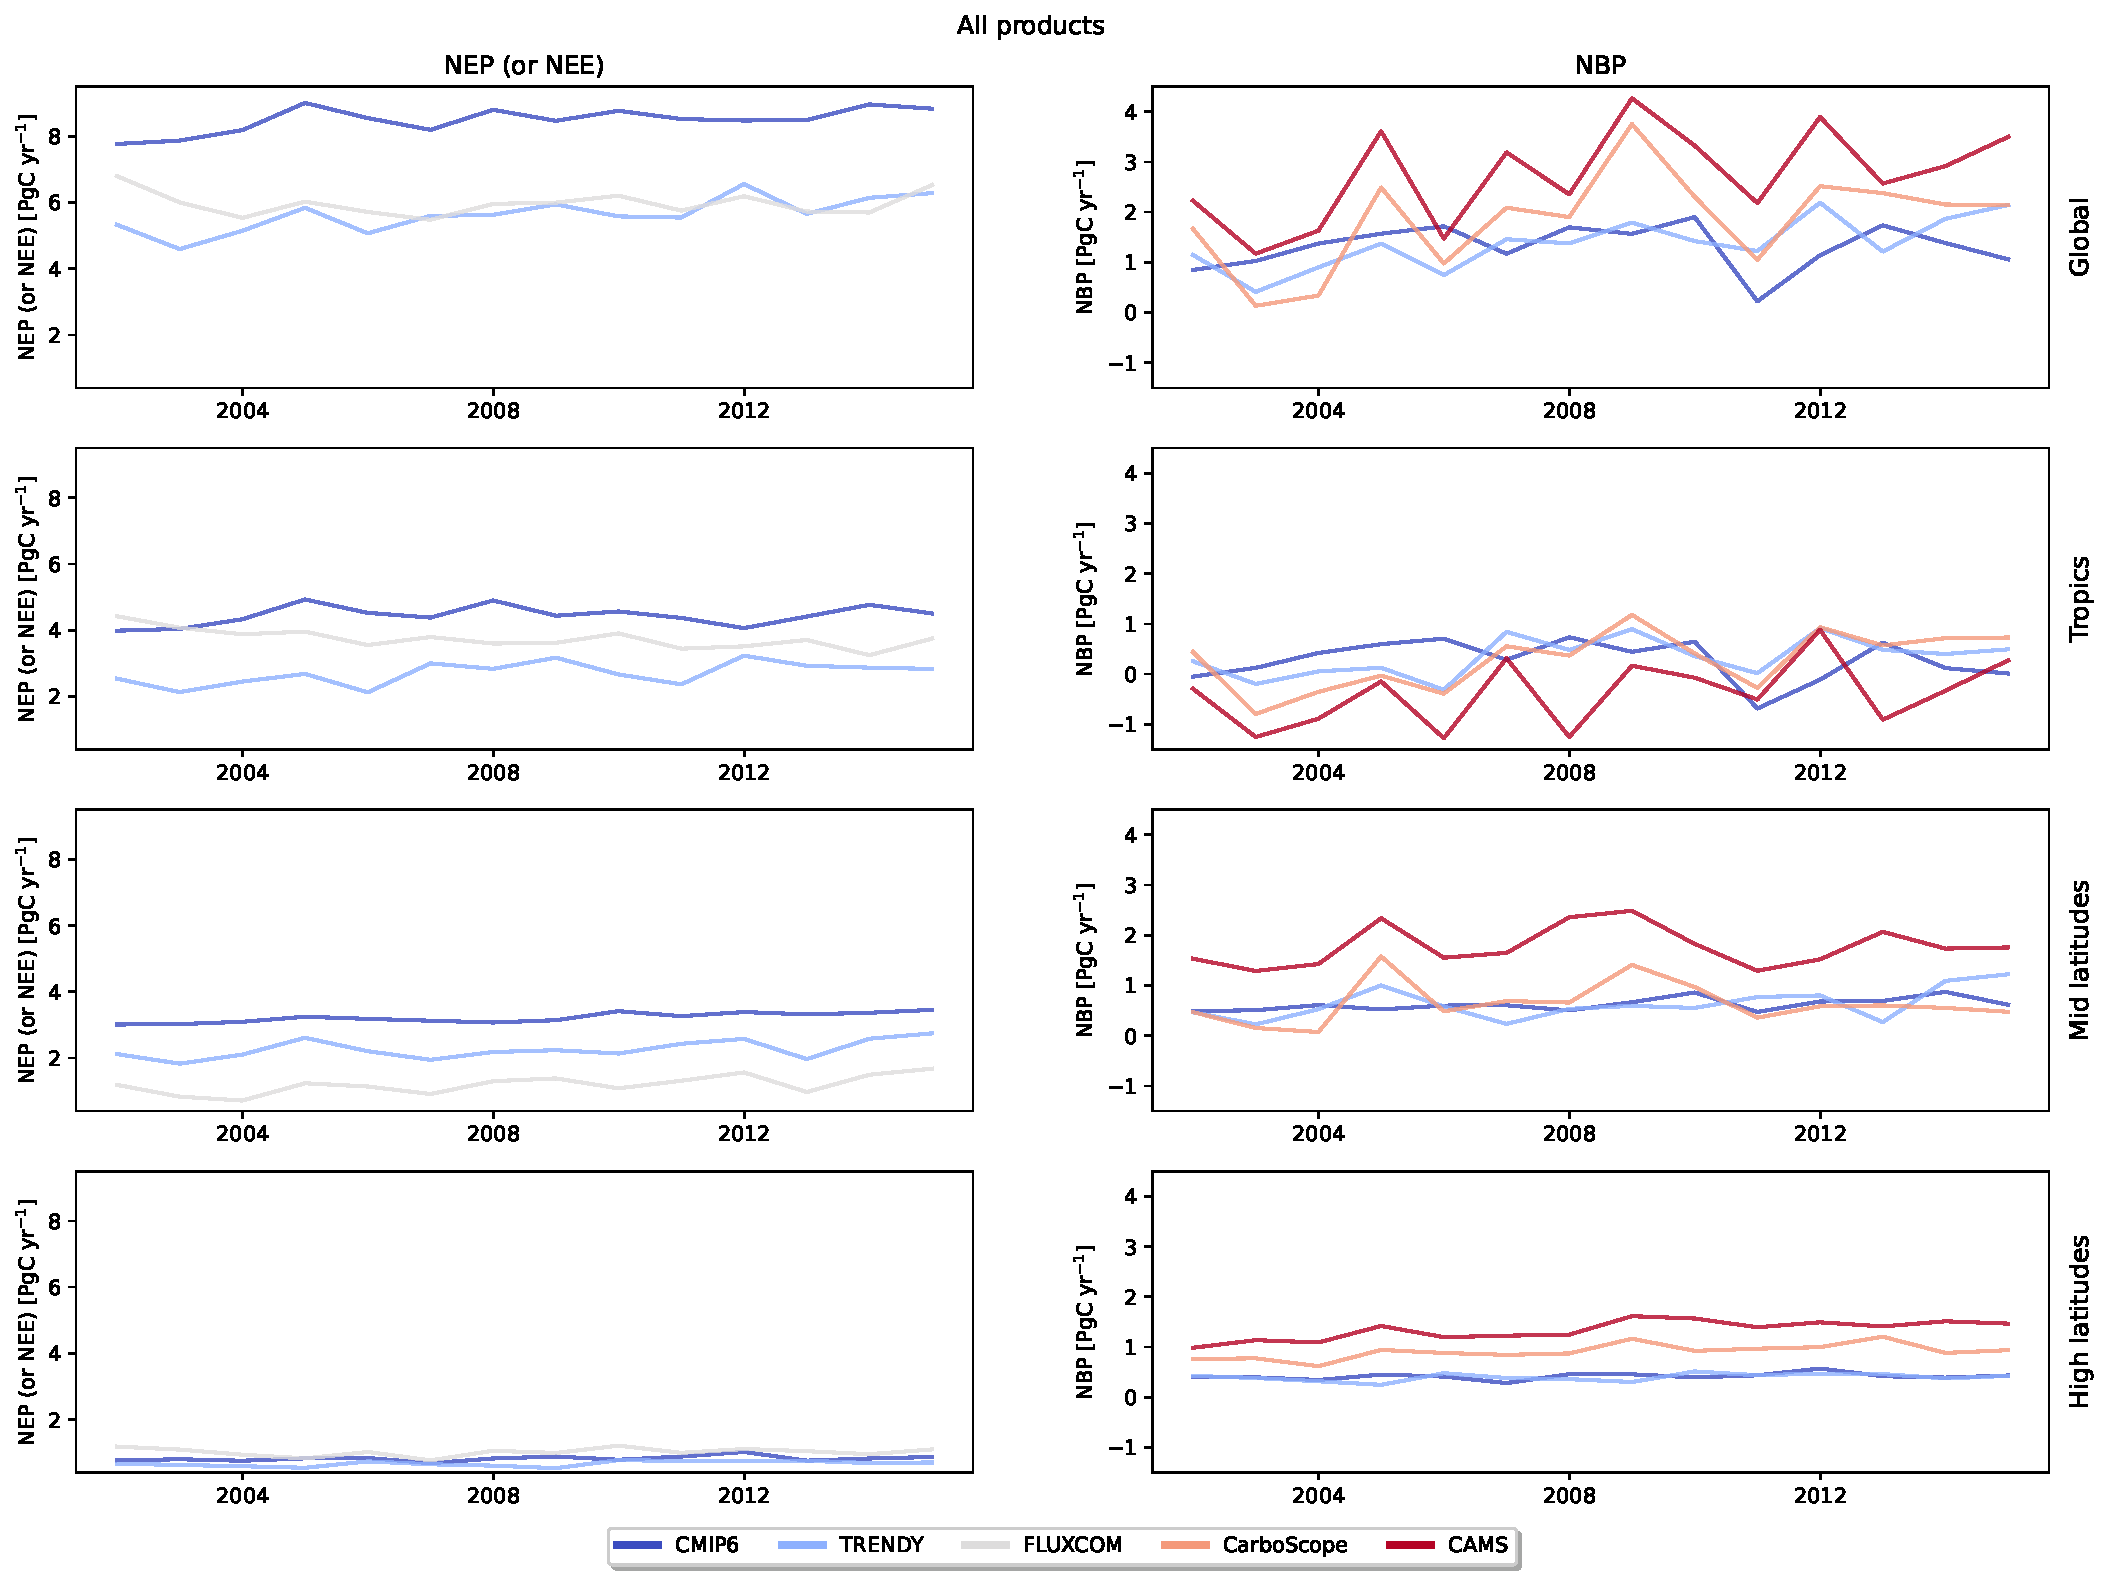
\includegraphics[width=1.0\linewidth]{Figures/Allproducts_variables.pdf}
    \caption{Time series of the annual mean of NEP (NEE for X-BASE) and NBP (vertical panels) from all products, cumulated globally, in the tropics, mid-latitudes, and high latitudes (horizontal panels). Colors indicate the different products.}
    \label{fig:vars_allprod}
\end{figure}

\section{Model weights}

\begin{figure}[H]
    \centering
    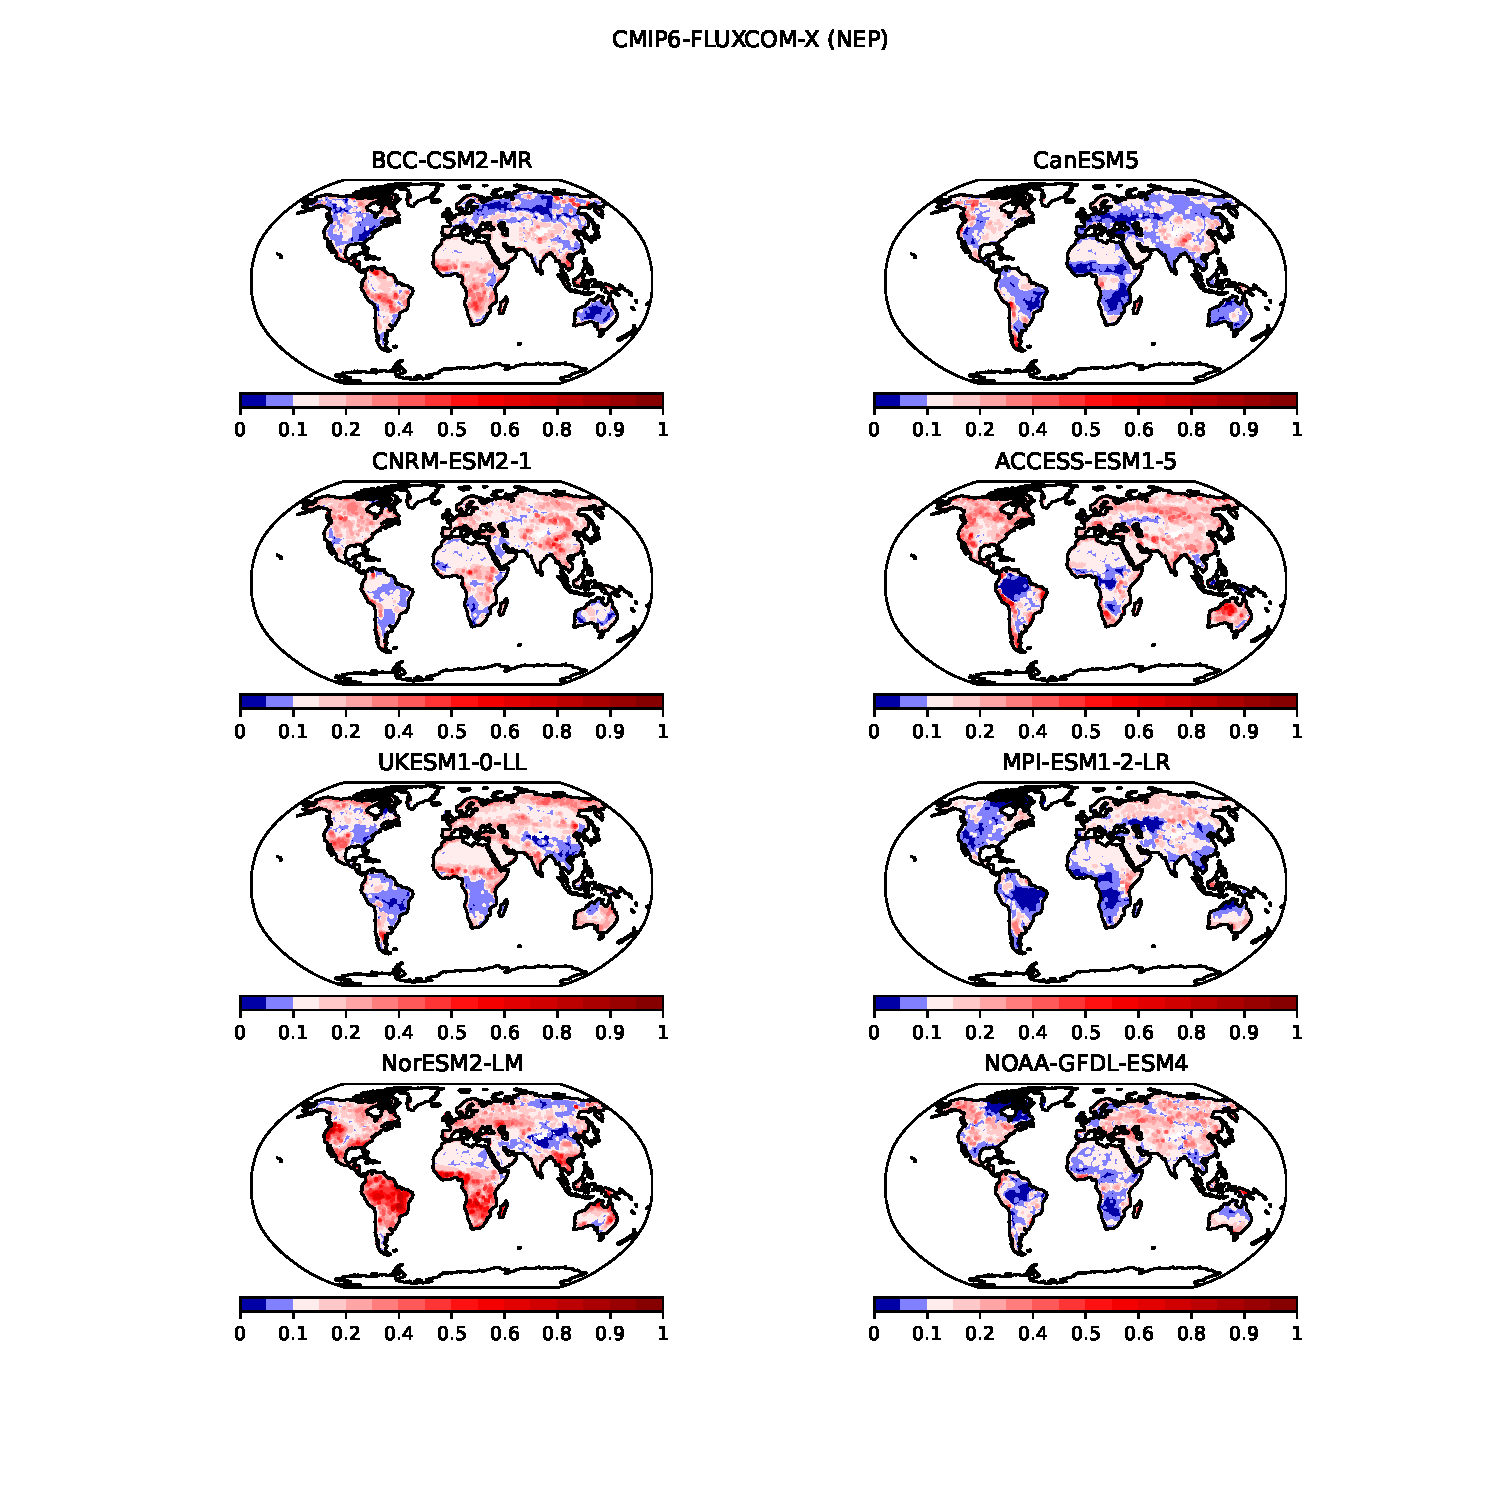
\includegraphics[width=1.0\linewidth]{Figures/CMIP6_FLUXCOM_weights.pdf}
    \caption{Spatial weights of NEP CMIP6 models to calculate the ensemble model average derived from X-BASE (NEE). Diverging color tables indicate whether the model contributes more or less than 1/8, where 8 is the number of models.}
    \label{fig:weights_CMIP6-FLUXCOMX}
\end{figure}

\newpage
\begin{figure}[H]
    \centering
    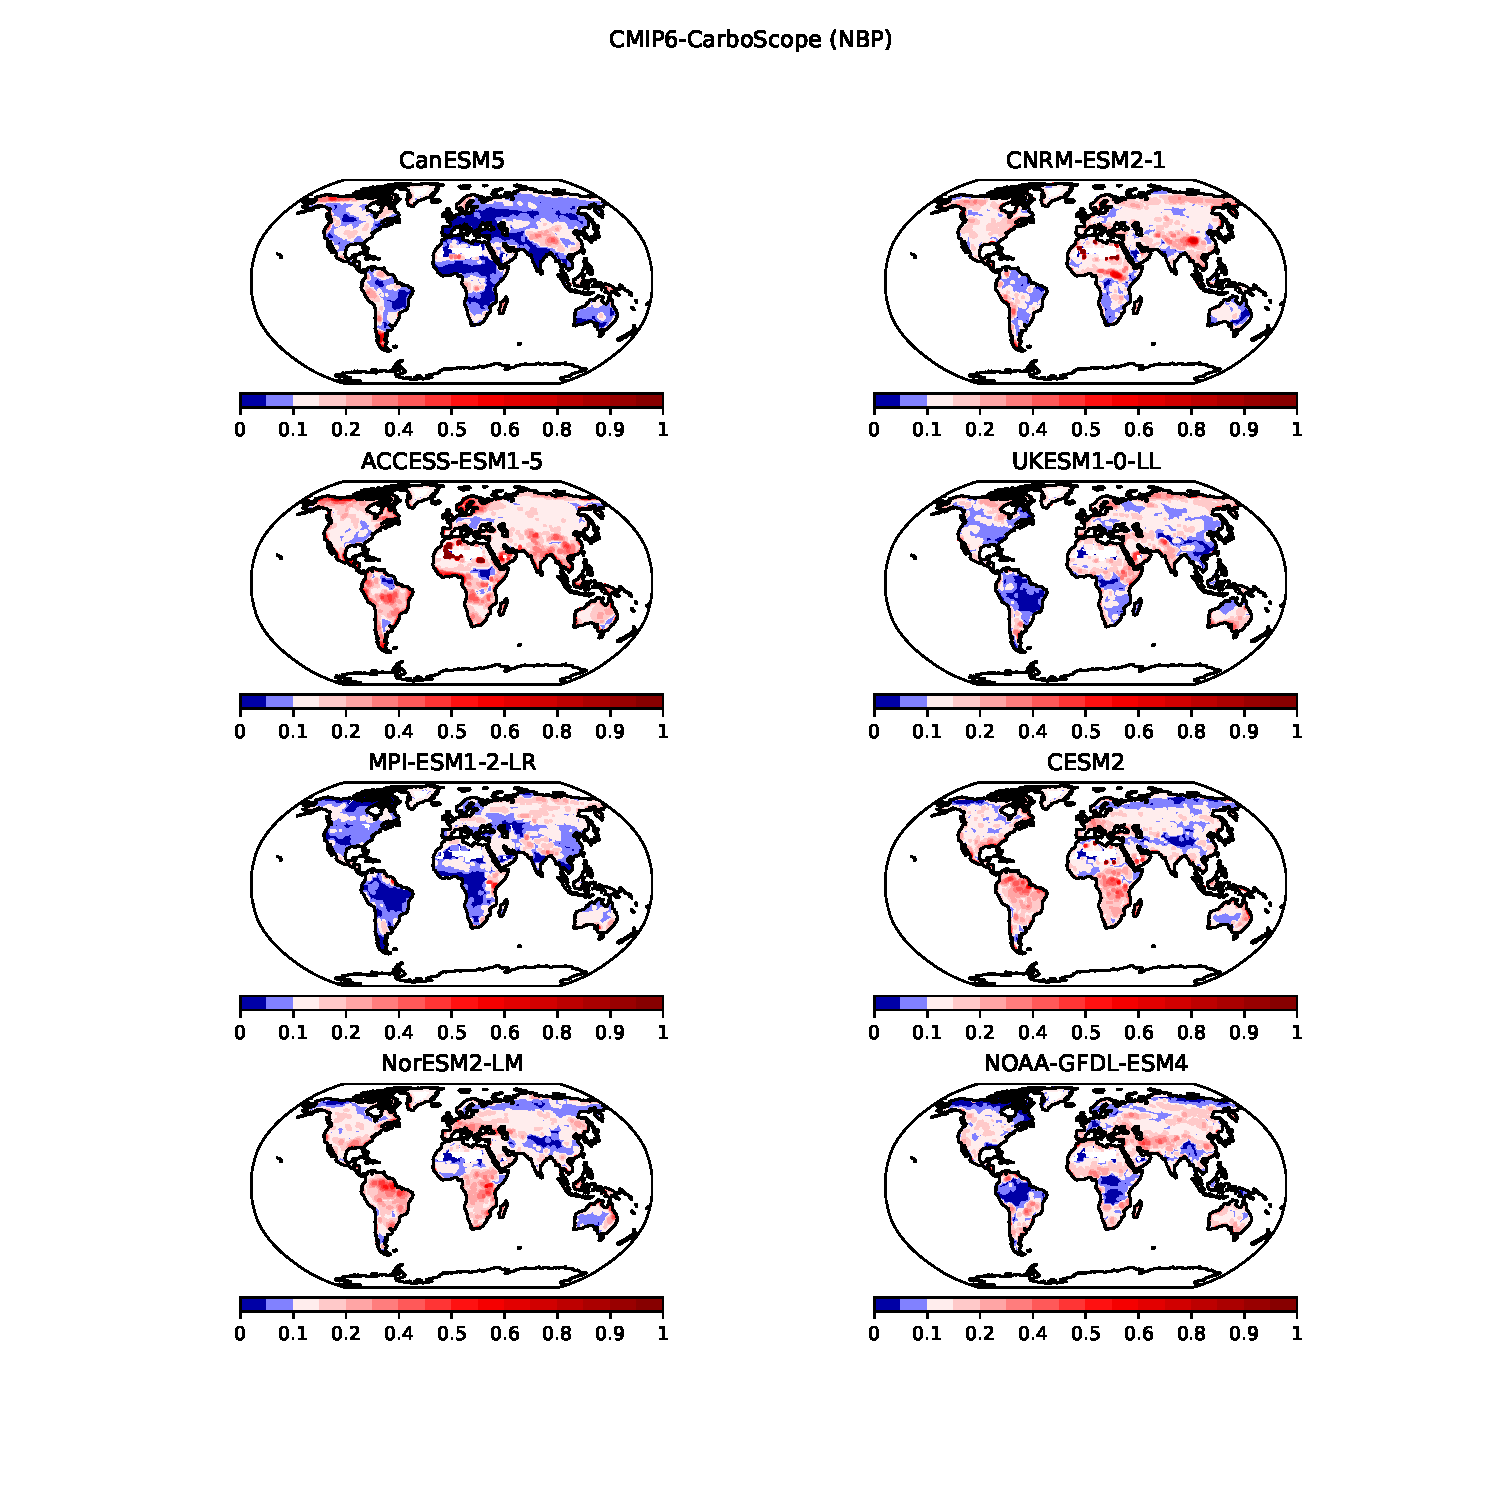
\includegraphics[width=1.0\linewidth]{Figures/CMIP6_CarboScope_weights.pdf}
    \caption{Spatial weights of NBP CMIP6 models to calculate the ensemble model average derived from CarboScope. Diverging color tables indicate whether the model contributes more or less than 1/8, where 8 is the number of models.}
    \label{fig:weights_CMIP6-CarboScope}
\end{figure}

\newpage

\begin{figure}[H]
    \centering
    \includegraphics[width=1.0\linewidth]{Figures/TRENDY_CarboScope_weights.pdf}
    \caption{Spatial weights of NEP TRENDY models to calculate the ensemble model derived from X-BASE (NEE). Diverging color tables indicate whether the model contributes more or less than 1/20, where 20 is the number of models.}
    \label{fig:weights_TRENDY-FLUXCOMX}
\end{figure}

\newpage

\begin{figure}[H]
    \centering
    \includegraphics[width=1.0\linewidth]{Figures/TRENDY_CarboScope_weights.pdf}
    \caption{Spatial weights of NBP TRENDY models to calculate the ensemble model derived from CarboScope. Diverging color tables indicate whether the model contributes more or less than 1/18, where 18 is the number of models.}
    \label{fig:weights_TRENDY-CarboScope}
\end{figure}


\section{Supplementary results}

\begin{table}[H]
\label{Table:CSdiff_NEP_NBP}
\centering
\begin{tabular}{lcccc}
\hline
\multicolumn{5}{c}{\textbf{CMIP6 1850-2014}}                                                                                       \\ \hline
\textbf{}                         & \textbf{Global}      & \textbf{Tropics}     & \textbf{Mid latitudes} & \textbf{High latitudes} \\
\textbf{CS NEP {[}PgC yr{]}}      & 72518              & 42810              & 25621                & 4088                 \\
\textbf{CS NBP {[}PgC yr{]}}      & -2841             & -912             & -1752               & -177               \\ \hline
\textbf{Difference  {[}PgC yr{]}} & \textbf{75359}     & \textbf{43721}     & \textbf{27373}       & \textbf{4265}        \\ \hline
                                  & \multicolumn{1}{l}{} & \multicolumn{1}{l}{} & \multicolumn{1}{l}{}   & \multicolumn{1}{l}{}    \\ \hline
\multicolumn{5}{c}{\textbf{CMIP6 2001-2014}}                                                                                       \\ \hline
\textbf{}                         & \textbf{Global}      & \textbf{Tropics}     & \textbf{Mid latitudes} & \textbf{High latitudes} \\
\textbf{CS NEP {[}PgC yr{]}}      & 820.11               & 426.78               & 310.86                 & 82.47                   \\
\textbf{CS NBP {[}PgC yr{]}}      & 139.41               & 33.17                & 62.57                  & 43.67                   \\
\textbf{Difference  {[}PgC yr{]}} & \textbf{680.70}      & \textbf{393.61}      & \textbf{248.29}        & \textbf{38.80}          \\ \hline
                                  & \multicolumn{1}{l}{} & \multicolumn{1}{l}{} & \multicolumn{1}{l}{}   & \multicolumn{1}{l}{}    \\ \hline
\multicolumn{5}{c}{\textbf{TRENDY 2001-2014}}                                                                                      \\ \hline
\textbf{}                         & \textbf{Global}      & \textbf{Tropics}     & \textbf{Mid latitudes} & \textbf{High latitudes} \\
\textbf{CS NEP {[}PgC yr{]}}      & 535.83               & 251.86               & 217.09                 & 66.88                   \\
\textbf{CS NBP {[}PgC yr{]}}      & 124.61               & 24.02                & 59.82                  & 40.78                   \\
\textbf{Difference  {[}PgC yr{]}} & \textbf{411.22}      & \textbf{227.84}      & \textbf{157.27}        & \textbf{26.11}          \\ \hline
\end{tabular}
\caption{CS values and differences between calculations based on NEP and NBP for CMIP6 during 1880-2014 and 2001-2014 and TRENDY during 2001-2014.}
\end{table}



\begin{figure}%[\sidecaptionrelwidth][t!]
    \centering
    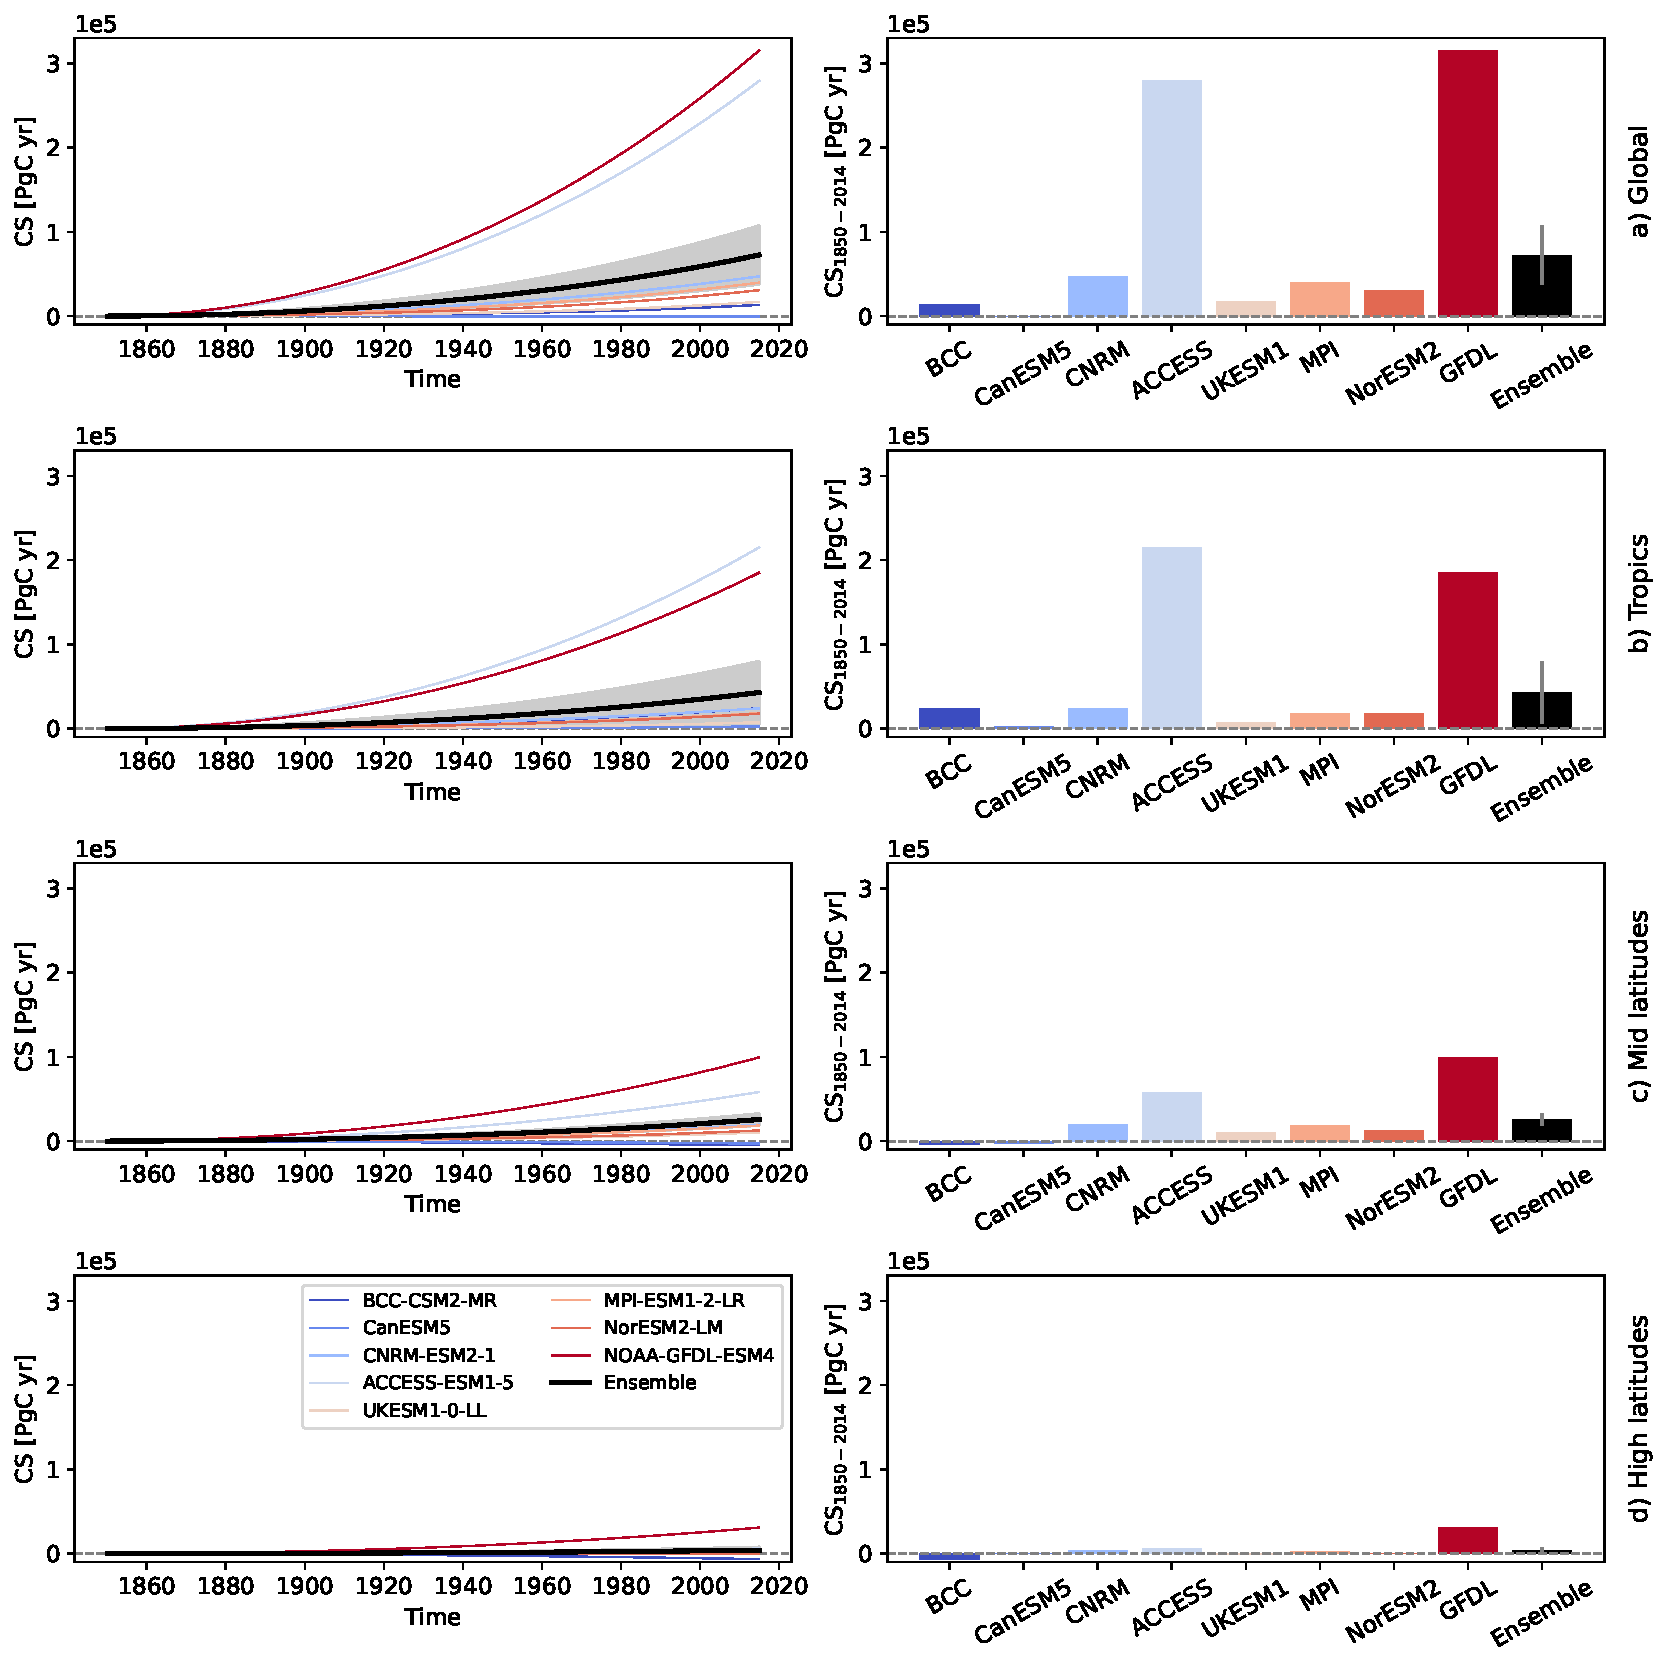
\includegraphics[width=1.0\linewidth]{Figures/CMIP6_NEP_CS_time_final.pdf}
    \caption{Time accumulation of Carbon Sequestration (CS) (left panel) and CS at the end of the period from 1850 to 2014 (right panel) calculated using NEP for a) global, b) tropics, c) mid-latitudes, and d) high-latitudes zones calculated using the results of 8 models from CMIP6. Black lines and bars indicate the results using the ensemble of the models. The dotted lines indicate null values of CS. The gray shaded area in the left column and the error bars in the right column represent the ensemble average $\pm$ the value of $\sigma$, calculated from the spread of all models. To save space, only the initial part of each model name is displayed on the horizontal axes in the right panel.}
    \label{fig:CMIP6_NEP_time_models}
\end{figure}

\begin{figure}
    \centering
    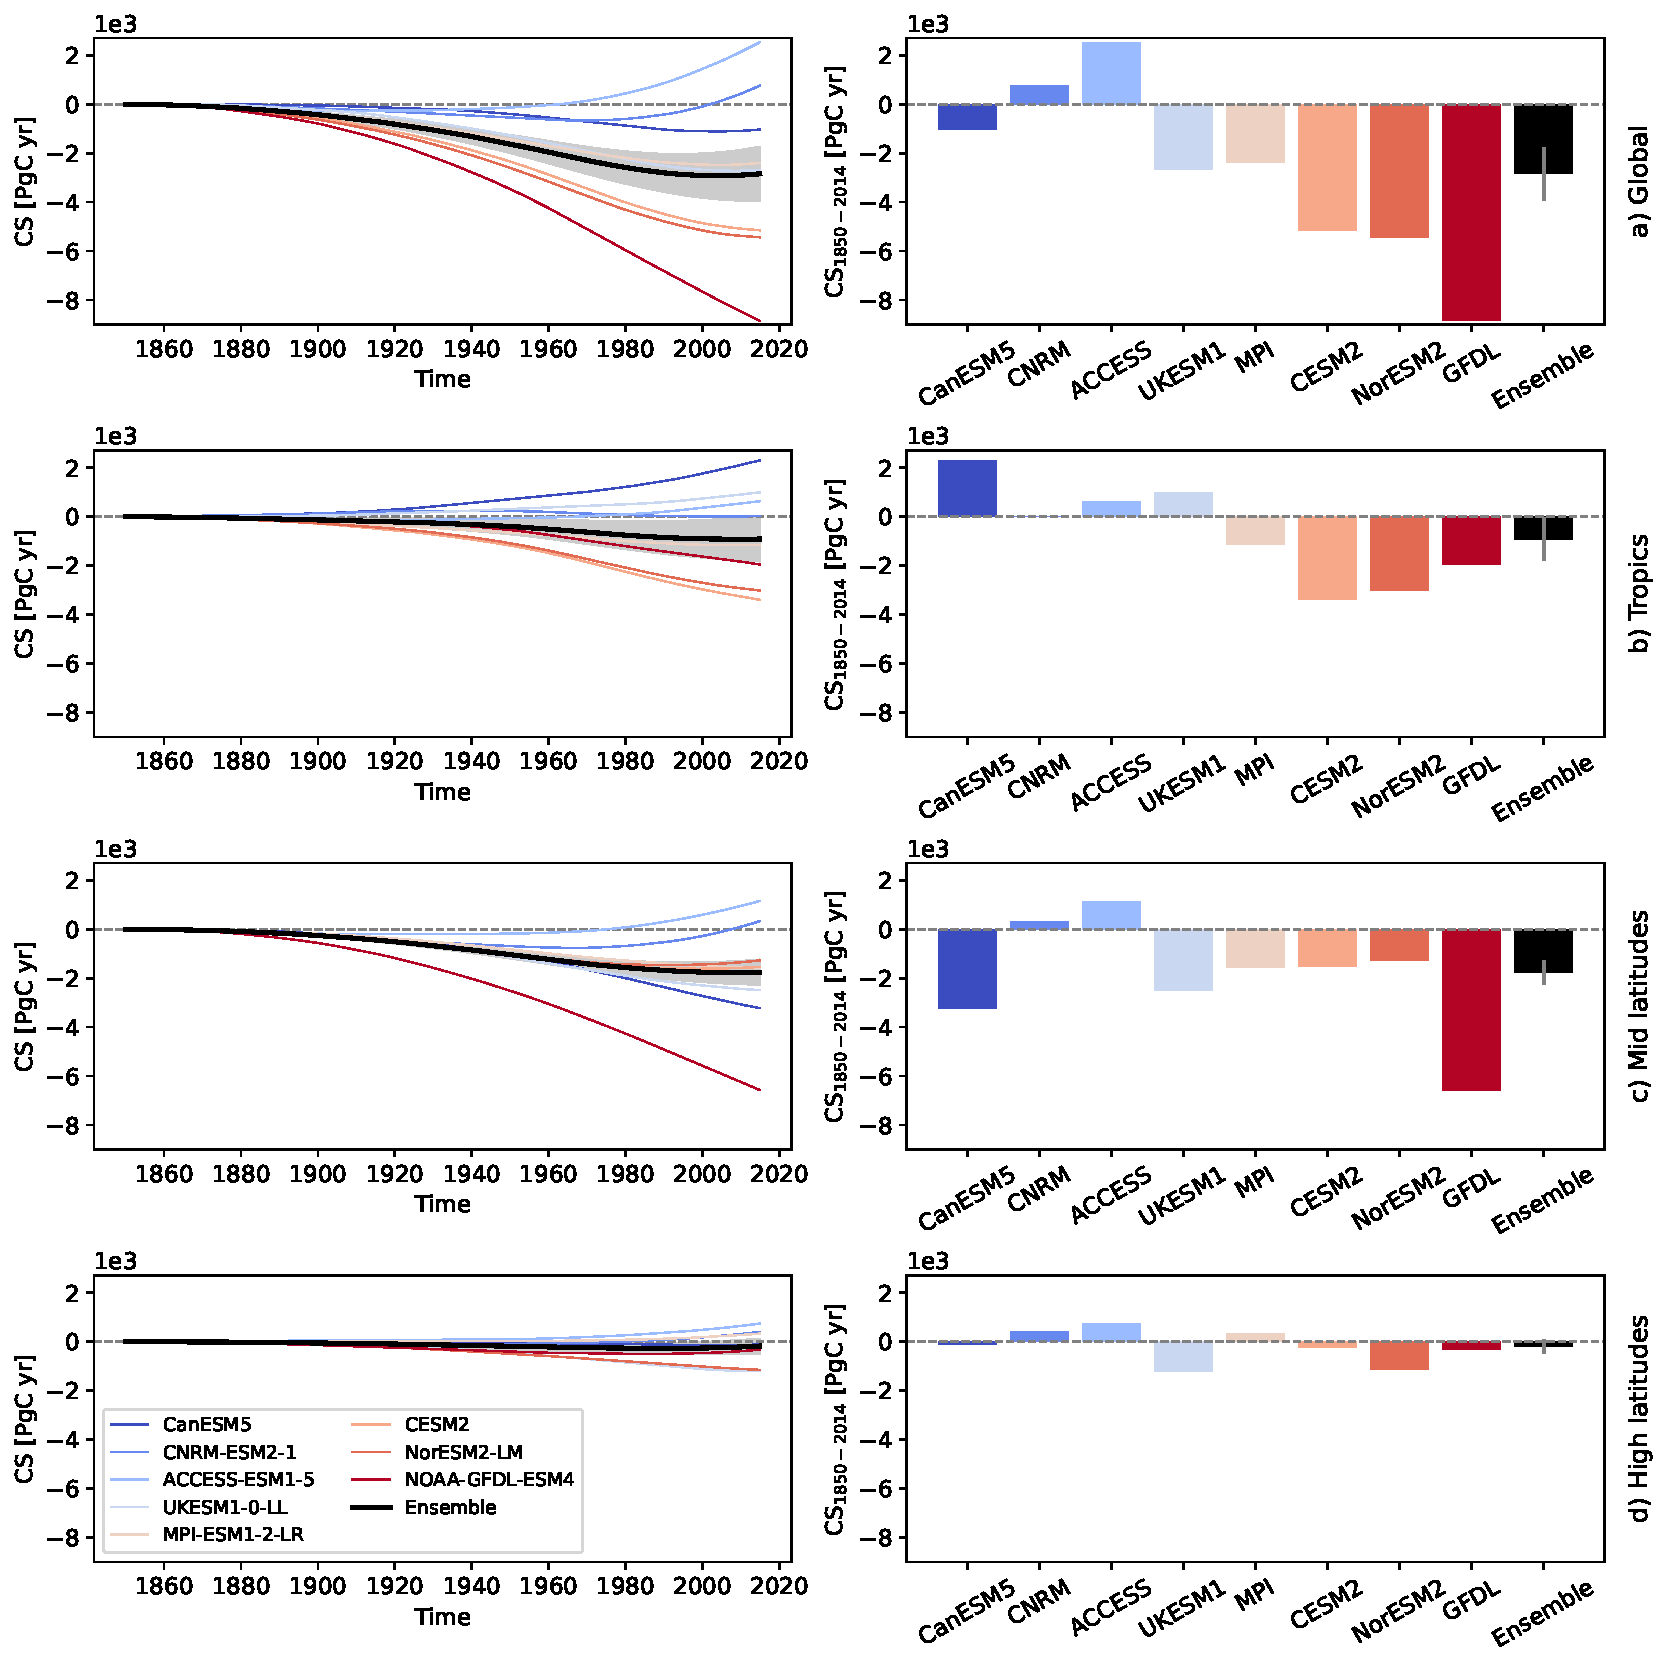
\includegraphics[width=1.0\linewidth]{Figures/CMIP6_NBP_CS_time_final.pdf}
    \caption{Time accumulation of Carbon Sequestration (CS) (left panel) and CS at the end of the period from 1850 to 2014 (right panel) calculated using NBP for a) global, b) tropics, c) mid-latitudes, and d) high-latitudes zones calculated using the results of 8 models from CMIP6. Black lines and bars indicate the results using the ensemble of the models. The dotted lines indicate null values of CS. The gray shaded area in the left column and the error bars in the right column represent the ensemble average $\pm$ the value of $\sigma$, calculated from the spread of all models. To save space, only the initial part of each model name is displayed on the horizontal axes in the right panel.}
    \label{fig:CMIP6_NBP_time_models}
\end{figure}

\begin{figure}
    \centering
    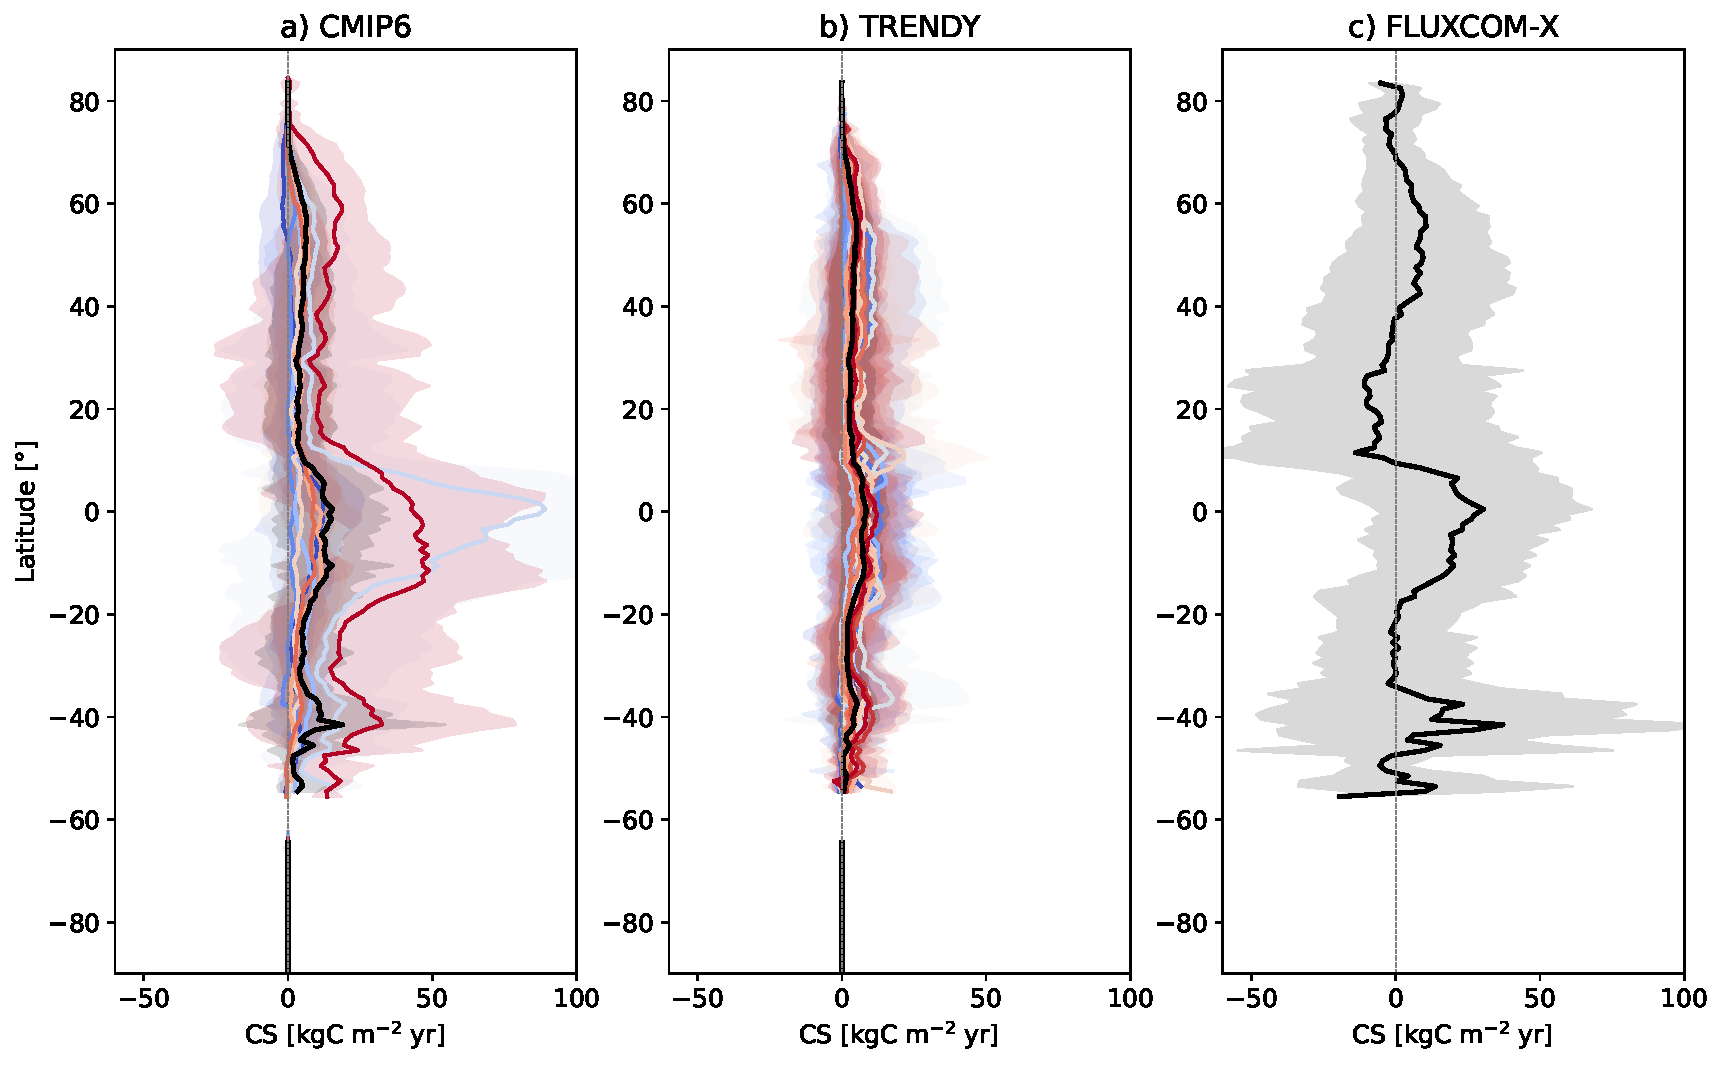
\includegraphics[width=1.0\linewidth]{Figures/Comparison_CS_latitude_NEP.pdf}
    \caption{Latitudinal CS profiles obtained from NEP (or NEE) from a) CMIP6, b) TRENDY, and c) X-BASE. Colored lines in a) and b) represent individual models; the black line is their ensemble. The dotted lines represent null carbon sequestration, and the shadow areas are two standard deviations from the mean.}
    \label{fig:LatCS_NEP}
\end{figure}


\begin{figure}
    \centering
    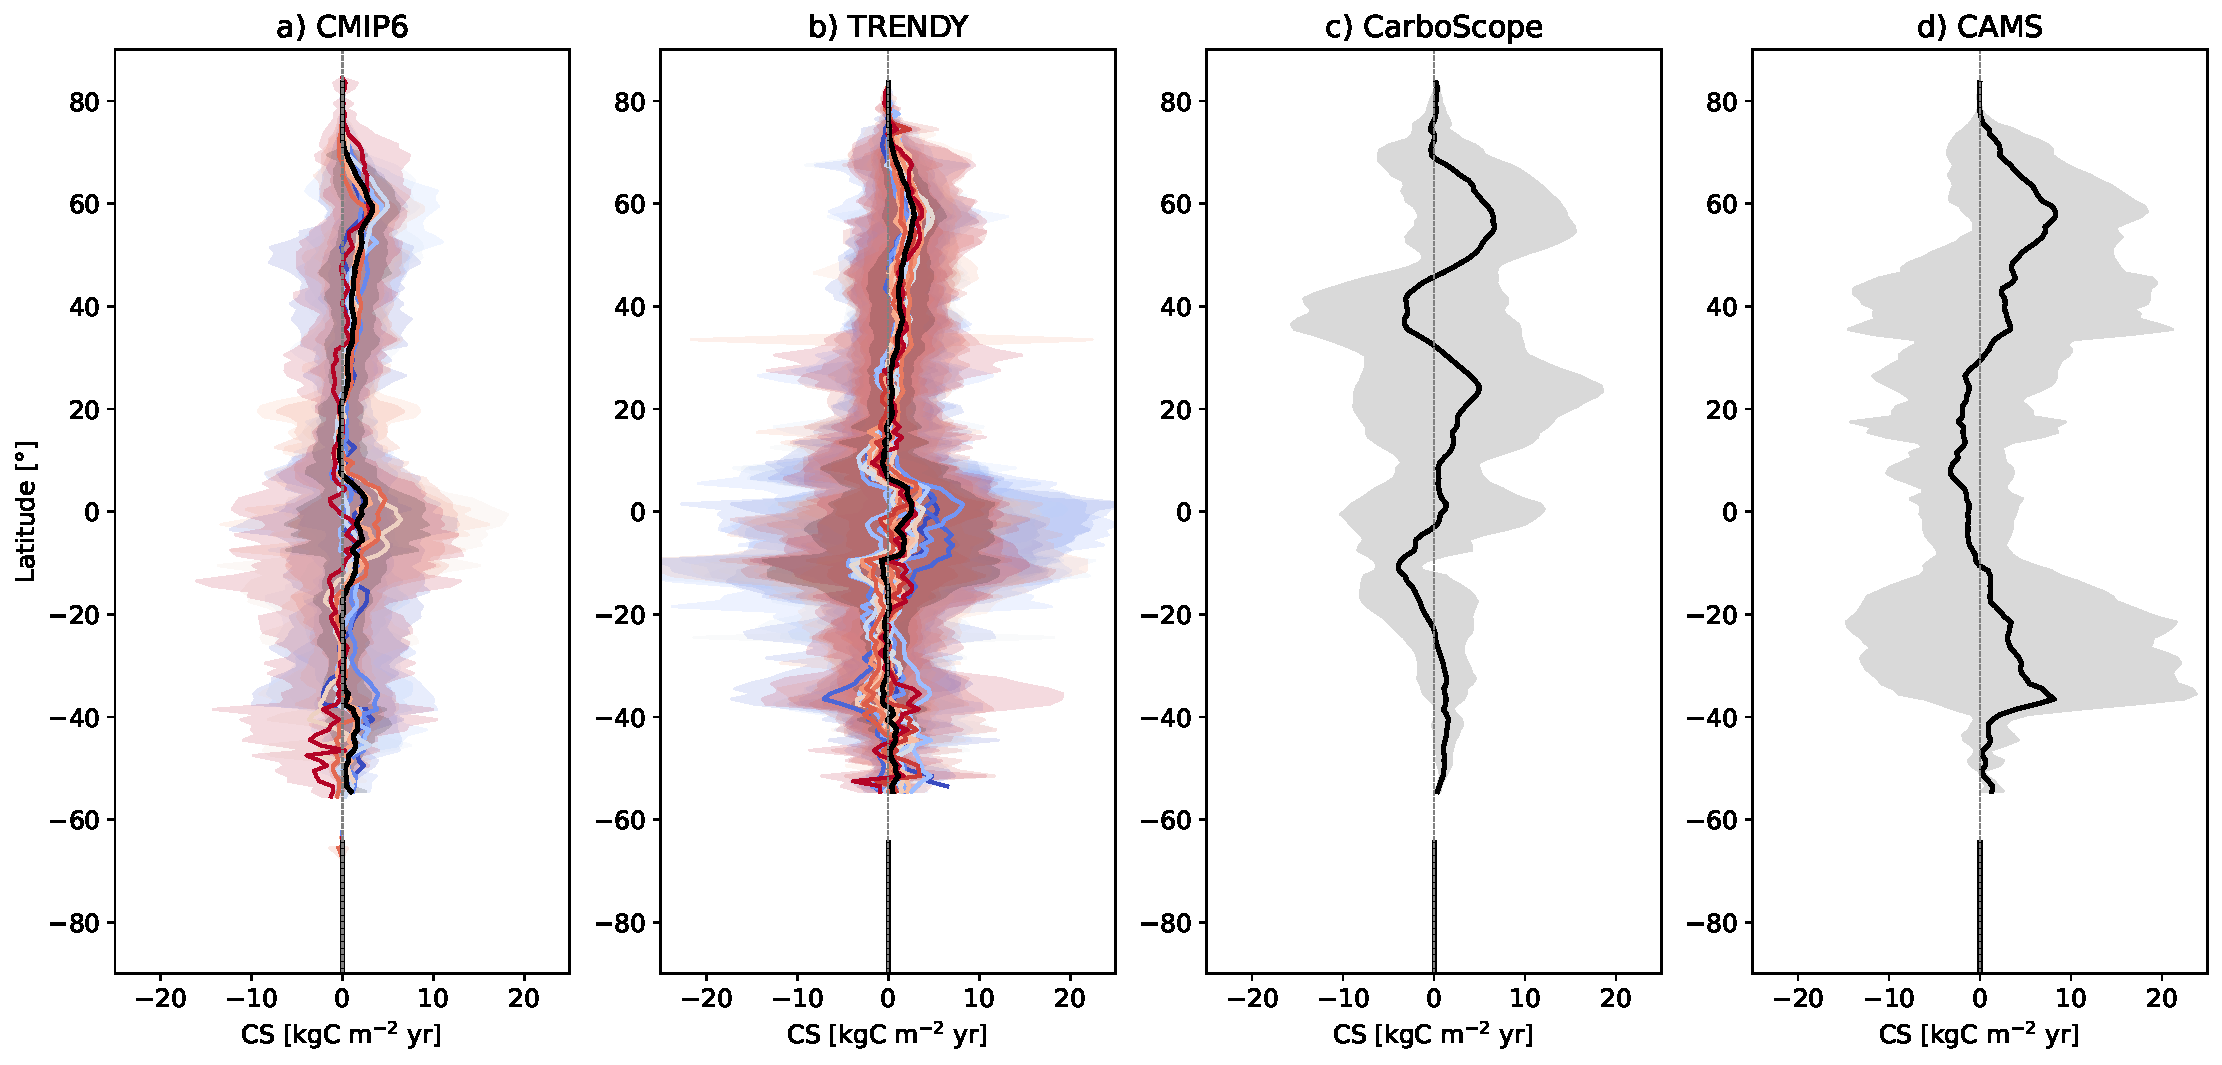
\includegraphics[width=1.0\linewidth]{Figures/Comparison_CS_latitude_NBP.pdf}
    \caption{Latitudinal CS profiles obtained from NBP from a) CMIP6, b) TRENDY, c) CarboScope, and d) CAMS. Colored lines in a) and b) represent individual models; the black line is their ensemble. The dotted lines represent null carbon sequestration, and the shadow areas are two standard deviations from the mean.}
    \label{fig:LatCS_NBP}
\end{figure}

\begin{figure}
    \centering
    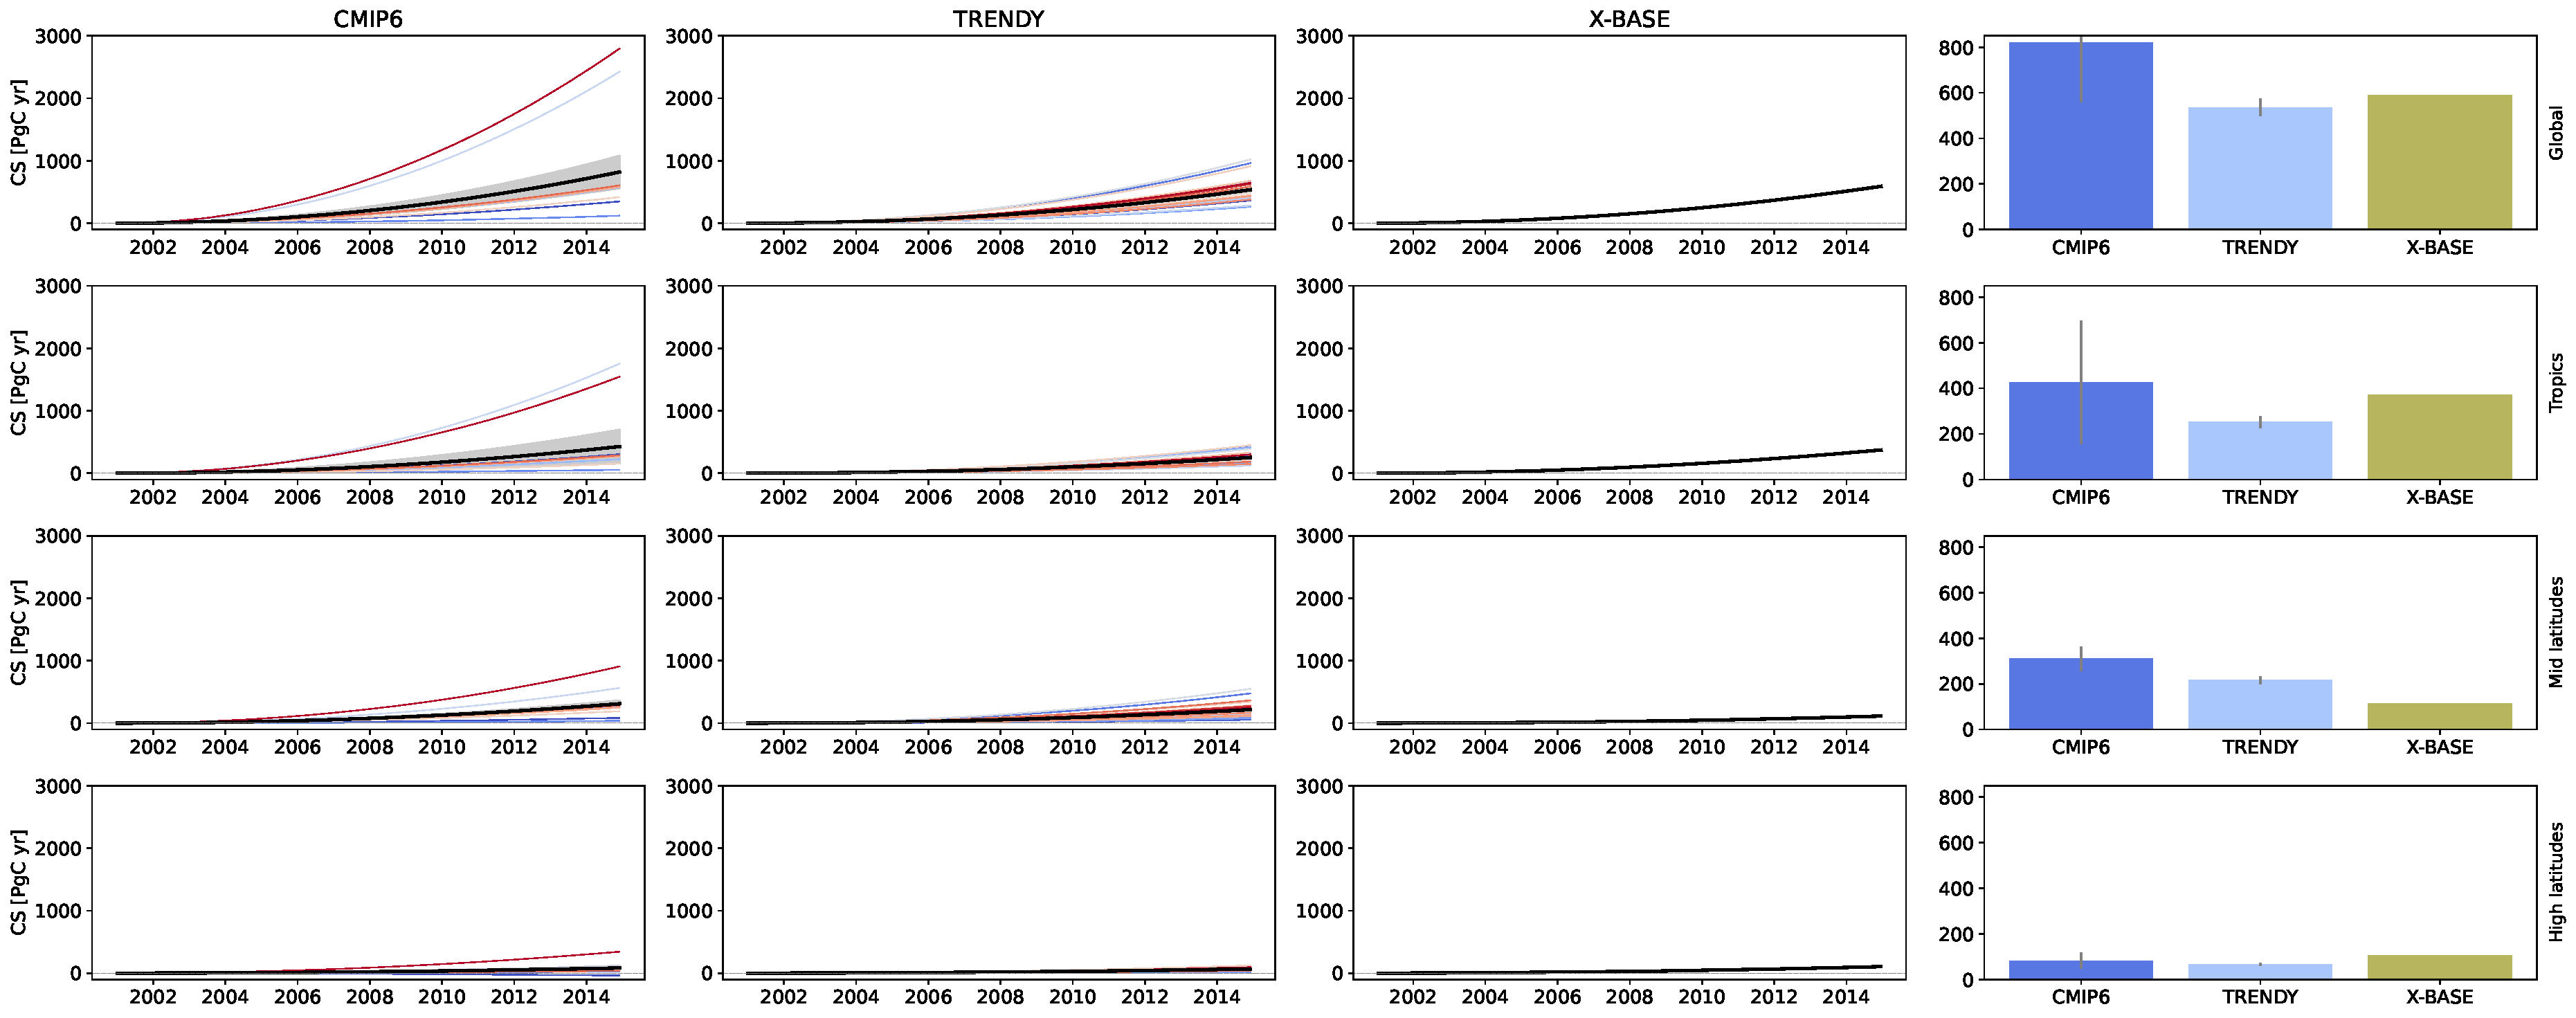
\includegraphics[width=1.0\linewidth]{Figures/Comparison_CS_temporal_NEP.pdf}
    \caption{Time accumulation of Carbon Sequestration (CS) of CMIP6 (1st vertical panel), TRENDY (2nd vertical panel), and X-BASE (3rd vertical panel), and CS at the end of the period from 2001 to 2014 (right panel) calculated using NEP (or NEE) for global (1st horizontal panel), tropics (2nd horizontal panel), mid-latitudes (3rd horizontal panel), and high-latitudes zones (4th horizontal panel). Black lines in the 1st and 2nd horizontal panels indicate the results using the ensemble of the models and bars for CMIP6 and TRENDY in the right panel, which correspond to their ensembles. The dotted lines indicate null values of CS. The gray shaded area in columns 1 and 2 and the error bars in column 4 represent the ensemble average $\pm$ the value of $\sigma$, calculated from the spread of all models from CMIP6 or TRENDY.}
    \label{fig:TempCS_NEP}
\end{figure}

\begin{figure}
    \centering
    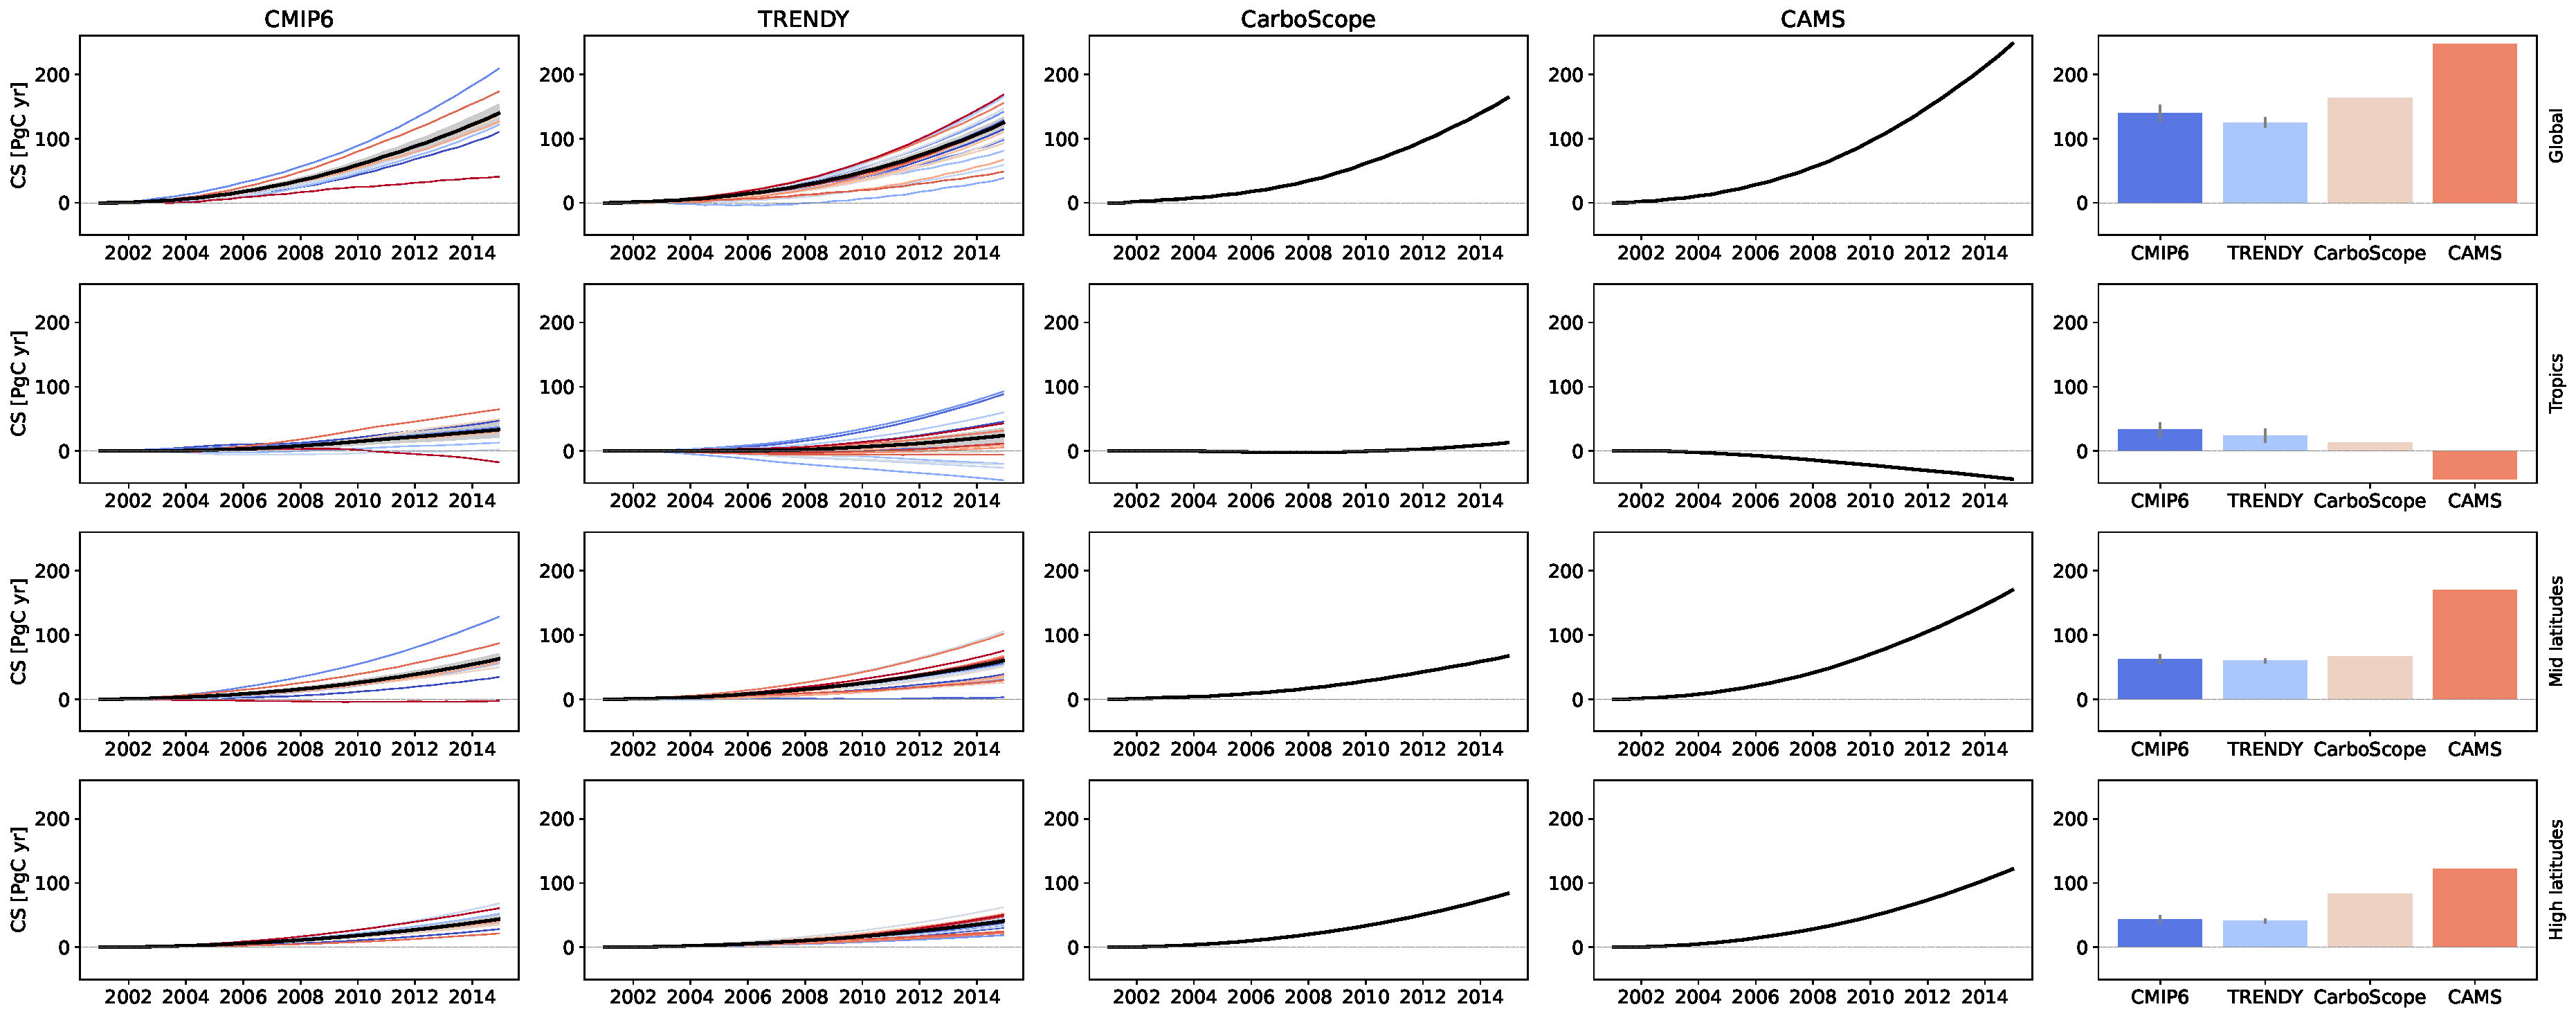
\includegraphics[width=1.0\linewidth]{Figures/Comparison_CS_temporal_NBP.pdf}
    \caption{Time accumulation of Carbon Sequestration (CS) of CMIP6 (1st vertical panel), TRENDY (2nd vertical panel), CarboScope (3rd vertical panel) and CAMS (4th vertical panel), and CS at the end of the period from 2001 to 2014 (right panel) calculated using NBP for global(1st horizontal panel), tropics (2nd horizontal panel), mid-latitudes (3rd horizontal panel), and high-latitudes zones (4th horizontal panel). Black lines in the 1st and 2nd panels indicate the results using the ensemble of the models and bars for CMIP6 and TRENDY in the right panel, which correspond to their ensembles. The dotted lines indicate null values of CS. The gray shaded area in columns 1 and 2 and the error bars in column 5 represent the ensemble average $\pm$ the value of $\sigma$, calculated from the spread of all models from CMIP6 or TRENDY.}
    \label{fig:TempCS_NBP}
\end{figure}


\begin{figure}
    \centering
    \includegraphics[width=1.0\linewidth]{Figures/CMIP6_Scatter_plots_res.pdf}
    \caption{Scatter plots of CS calculated from NEP (odd columns) and NBP (even columns) versus dependent variables: GPP (columns 1-2), respiration ($R_e=r_a+r_h$, columns 3-4), NEP (columns 5-6) and NBP (columns 7-8) for each model. Each row represents a specific CMIP6, and the data points are colored to indicate the different latitudinal regions.}
    \label{fig:scatter_CMIP6}
\end{figure}




%%% Add this line AFTER all your figures and tables
\FloatBarrier

% \movie{Type legend for the movie here.}

% \movie{Type legend for the other movie here. Adding longer text to show what happens, to decide on alignment and/or indentations.}

% \movie{A third movie, just for kicks.}

% \dataset{dataset_one.txt}{Type or paste legend here.}

% \dataset{dataset_two.txt}{Type or paste legend here. Adding longer text to show what happens, to decide on alignment and/or indentations for multi-line or paragraph captions.}

\bibliography{biblio}

\end{document}
